\chapter{Flow-Based Perspective: From NFs to Flow Matching}\label{ch:flow-based}


\epigraph{
    \textit{Everything flows.
}}{Heraclitus}


The \emph{change-of-variables formula}, a cornerstone of probability
theory~\citep{tabak2010density,tabak2013family}, takes on new life in modern
generative modeling. In \Cref{ch:score-sde}, we saw that the Fokker--Planck
equation describes how probability densities evolve under a diffusion process,
and that the same marginal density evolution can also be realized
deterministically through the associated PF-ODE. This naturally suggests
studying generative modeling directly from the viewpoint of deterministic
probability transport.

\paragraph{Change-of-Variables Formula of Densities.}
Given an invertible transformation $\rvf$, the density of
$\rvx=\rvf(\rvz)$, where $\rvz\sim p_{\mathrm{prior}}$, is
\begin{mdframed}
\begin{align}\label{eq:nf-change-of-var}
p(\rvx)
=
p_{\mathrm{prior}}(\rvz)
\left|
\det
\frac{\partial \rvf^{-1}(\rvx)}{\partial \rvx}
\right|,
\qquad
\text{where }
\rvz=\rvf^{-1}(\rvx).
\end{align}
\end{mdframed}
This deceptively simple formula enables bidirectional transport of samples and
densities when $\rvf$ is tractable, forming the foundation of Normalizing
Flows, which we introduce in \Cref{sec:flow-based-method}. But what happens
when this transformation is viewed continuously in time?

In this chapter, we follow this idea from Normalizing Flows to Neural ODEs and
then to Flow Matching. The key connection to \Cref{ch:score-sde} is especially
important. In Score SDEs, the learned score is used to construct the velocity field of
the PF-ODE. Flow Matching instead learns a velocity field directly. For the
same diffusion probability path, these provide two views of the same
deterministic probability flow.

A useful mental picture for this chapter is therefore, where both rely on the same conditioning principle:



\begin{figure}[th!]
\centering
\newcommand{\subnote}[1]{{\scriptsize\itshape\textcolor{black!62}{#1}}}
\resizebox{\ifdim\width>\linewidth \linewidth\else \width\fi}{!}{%
\begin{tikzpicture}[
  font=\small,
  >={Latex[length=2.4mm,width=1.7mm]},
  block/.style={rectangle, rounded corners=2pt, line width=.6pt, align=center,
                text width=3.6cm, inner sep=6pt, minimum height=1.25cm},
  sblock/.style={block, draw=scoreblue!75, fill=scoreblue!7},
  fblock/.style={block, draw=fmorange!75,  fill=fmorange!7},
  bridge/.style={block, draw=black!70, fill=white, line width=.8pt},
  shared/.style={block, draw=black!75, fill=black!5, line width=.9pt},
  panel/.style={rounded corners=5pt, line width=.7pt},
  head/.style={font=\footnotesize, inner sep=4pt, fill=white},
  arr/.style={->, semithick, black!60},
  lbl/.style={draw=black!25, rounded corners=2pt, fill=white, inner sep=3pt,
              font=\footnotesize, align=center}
]
 
%--------------------------- conditional row (what is regressed) ------------
\node[sblock] (cs) at (-3.0,2.55)
  {\textbfs{Conditional Score}\\[1pt]
   $\nabla_{\rvx}\log p_t(\rvx\,|\,\rvx_0)$\\[1pt]
   \subnote{closed form}};
 
\node[fblock] (cv) at (3.0,2.55)
  {\textbfs{Conditional Velocity}\\[1pt]
   $\rvv_t(\rvx\,|\,\rvz)$\\[1pt]
   \subnote{closed form}};
 
%--------------------------- marginal row (what is wanted) ------------------
\node[sblock] (ms) at (-3.0,0)
  {\textbfs{Marginal Score}\\[1pt]
   $\nabla_{\rvx}\log p_t(\rvx)$\\[1pt]
   \subnote{intractable}};
 
\node[fblock] (mv) at (3.0,0)
  {\textbfs{Marginal Velocity}\\[1pt]
   $\rvv_t(\rvx)$\\[1pt]
   \subnote{intractable}};
 
%--------------------------- panels (background) ----------------------------
\begin{pgfonlayer}{background}
  \node[panel, draw=scoreblue!40, fill=scoreblue!4,
        fit=(cs)(ms), inner xsep=8pt, inner ysep=12pt] (panelS) {};
  \node[panel, draw=fmorange!40, fill=fmorange!4,
        fit=(cv)(mv), inner xsep=8pt, inner ysep=12pt] (panelF) {};
\end{pgfonlayer}
 
\node[head, text=scoreblue] at (panelS.north) {\textbfs{Score SDE}};
\node[head, text=fmorange]  at (panelF.north) {\textbfs{Flow Matching}};
 
\draw[dashed, black!22, line width=.5pt]
  ($(panelS.north east)!0.5!(panelF.north west)$) --
  ($(panelS.south east)!0.5!(panelF.south west)$);
\node[fill=white, inner sep=2pt, text=black!45, font=\large]
  at ($(panelS.east)!0.5!(panelF.west)$) {$\Longleftrightarrow$};
 
%--------------------------- conditional averaging --------------------------
\draw[arr] (cs) -- (ms);
\draw[arr] (cv) -- (mv);
\node[lbl] at ($(cs)!0.5!(ms)$) {$\E_{\rvx_0\,|\,\rvx}\big[\,\cdot\,\big]$};
\node[lbl] at ($(cv)!0.5!(mv)$) {$\E_{\rvz\,|\,\rvx}\big[\,\cdot\,\big]$};
 
%--------------------------- the single conversion --------------------------
\node[bridge, text width=5.8cm] (conv) at (0,-3.45)
  {$\displaystyle \rvv_t(\rvx)=f(t)\rvx-\tfrac{1}{2}g^{2}(t)\,\nabla_{\rvx}\log p_t(\rvx)$};
 
% both columns drop, run together on a common bus, then one arrow descends
\coordinate (bus) at ($(panelS.south)+(0,-0.75)$);
\coordinate (busC) at (bus -| conv.north);
\draw[semithick, black!60, rounded corners=4pt] (panelS.south) |- (busC);
\draw[semithick, black!60, rounded corners=4pt] (panelF.south) |- (busC);
\draw[arr] (busC) -- (conv.north);
 
%--------------------------- shared destination -----------------------------
\node[shared, text width=7.8cm] (ode) at (0,-5.75)
  {\textbfs{The same probability flow}\\[4pt]
   $\displaystyle \frac{\diff \rvx(t)}{\diff t}=\rvv_t\big(\rvx(t)\big),$ \\[4pt] transporting between $p_{\mathrm{data}}$ and $p_{\mathrm{prior}}$.};
 
\draw[arr] (conv.south) -- (ode.north);
 
\end{tikzpicture}}
\caption{\textbfs{Score SDEs and Flow Matching.}
Both frameworks train on the closed-form \emph{conditional} quantity in the top
row. Averaging it over the conditioning variable (vertical arrows) gives the
intractable \emph{marginal} quantity below, which is what the trained model
recovers. The columns differ only in which quantity that is. On a diffusion
path the score determines the velocity through the conversion in the middle, so
both routes end at the same ODE; Flow Matching learns that velocity directly and
needs neither endpoint to be Gaussian.
\figcredit{Created by the authors.}}
\label{fig:score-fm-mental-picture}
\end{figure}

Flow Matching carries this principle beyond the usual Gaussian diffusion
setting. It can construct continuous transport between more general source and
target distributions from which samples are available, provided that the
chosen conditional probability paths can be sampled efficiently and their
conditional velocities can be computed tractably.

To support a solid understanding of this chapter, we provide in
\Cref{app:continuity} an intuitive, self-contained overview of the different
forms of the change-of-variables principle, progressing from the ordinary
change-of-variables formula to the continuity equation and, with stochastic
dynamics, to the Fokker--Planck equation.

\chapterlearning{
  \item connect Normalizing Flows, Neural ODEs, and Flow Matching through the common idea of transporting probability distributions, from discrete invertible transformations to continuous-time velocity fields;
  \item recognize the key analogy with the Score SDE framework in \Cref{ch:score-sde}: for the same diffusion probability path, Score SDEs learn a score that determines the PF-ODE velocity, whereas Flow Matching can learn that velocity field directly; in both cases, an intractable marginal target can be learned through tractable conditional targets;
  \item understand the continuity equation as the density-level rule that connects an ODE velocity field to the evolution of its probability distribution;
  \item understand how Flow Matching extends this conditional strategy beyond Gaussian diffusion paths to transport between general source and target distributions from which samples are available, while retaining simulation-free training through tractable conditional paths and velocities;
  \item distinguish the prescribed probability path $\{p_t\}_{t\in[0,1]}$ from the particular velocity field, coupling, and particle trajectories used to realize it, and understand why different flows can share the same marginal distributions;
  \item understand the two complementary ways of constructing tractable conditional flows: starting from a conditional probability path and deriving its velocity, or starting from a conditional flow map and deriving its velocity along trajectories.
}{
Readers already comfortable with Normalizing Flows and Neural ODEs may skim
\Cref{sec:flow-based-method} and begin with \Cref{subsec:lesson-score}.
For a first pass, focus on the connection between the Score SDE and Flow
Matching views, the continuity equation, and the conditional-to-marginal
velocity construction. The detailed path constructions and optional theoretical
properties can be revisited afterward.
}


\newpage

\section{Flow-Based Models: Normalizing Flows and Neural ODEs}\label{sec:flow-based-method}
In this section, we will introduce Flow-Based Models, including Normalizing Flows (NFs)~\citep{rezende2015variational} and Neural Ordinary Differential Equations (NODEs)~\citep{chen2018neural}.

NFs enable flexible and tractable probability density estimation by applying a series of invertible transformations to a simple base distribution. NODEs extend this framework to continuous time, where the transformation is governed by an ODE. By treating the transformations as continuous-time dynamics, NODEs provide a smooth, scalable extension to the NF paradigm.




% \vspace{0.4cm}
% \begin{figure}[tbh!]
%     \centering
%     \resizebox{\textwidth}{!}{ % resize entire figure to fit page width
%     \begin{tikzpicture}[
%         % --- Merged styles from your example ---
%         ->,                      % Sets default path to be an arrow
%         >=Stealth,               % Sets the arrowhead style to "Stealth"
%         thick,                   % Sets default line thickness
%         % font=\small,             % Sets default font size for nodes
%         % --- Existing styles ---    
%         % Style for the large function blocks
%         block/.style={
%             rectangle,
%             rounded corners=3pt,
%             draw=black,
%             fill=gray!20,
%             minimum width=1.5cm,
%             minimum height=1.5cm,
%             text width=2cm,
%             align=center,
%             % font=\scriptsize, % smaller text
%         },
%         % Style for x, z, and x' nodes (larger square blocks)
%         var_block/.style={
%             rectangle,
%             rounded corners=3pt,
%             draw=black,
%             fill=gray!20,
%             minimum size=1.2cm, % larger square size
%             align=center,
%         },
%         % Arrow styling
%         arrow/.style={-Stealth, thick}
%     ]

%     % Nodes
%     \node[var_block] (x_in) {$\rvx$};
%     \node[block, right=1.5cm of x_in] (fwd_func) {Inverse \\ Functions \\ $\rvf^{-1}(\rvx)$};
%     \node[var_block, right=1.5cm of fwd_func] (z_latent) {$\rvz$};
%     \node[block, right=1.5cm of z_latent] (inv_func) {  \\ Functions \\ $\rvf(\rvz)$};
%     \node[var_block, right=1.5cm of inv_func] (x_out) {$\rvx'$};

%     % Arrows
%     \draw[arrow] (x_in.east) -- (fwd_func.west);
%     \draw[arrow] (fwd_func.east) -- (z_latent.west);
%     \draw[arrow] (z_latent.east) -- (inv_func.west);
%     \draw[arrow] (inv_func.east) -- (x_out.west);

%     \end{tikzpicture}
%     }
%     \caption{Illustration of a NF. It consists of a sequence of invertible functions $\rvf: \rvz \mapsto \rvx$ that transform latent variable $\rvz$ into a data $\rvx$, together with the inverse mapping $\rvf^{-1}: \rvx \mapsto \rvz$ that reconstructs the data. An NF resembles an encoder--decoder structure, but with the encoder realized as a smooth invertible map and the decoder given exactly by its inverse.}
%     \label{fig:forward_inverse_diagram}
% \end{figure}


\begin{figure}[th!]
    \centering
    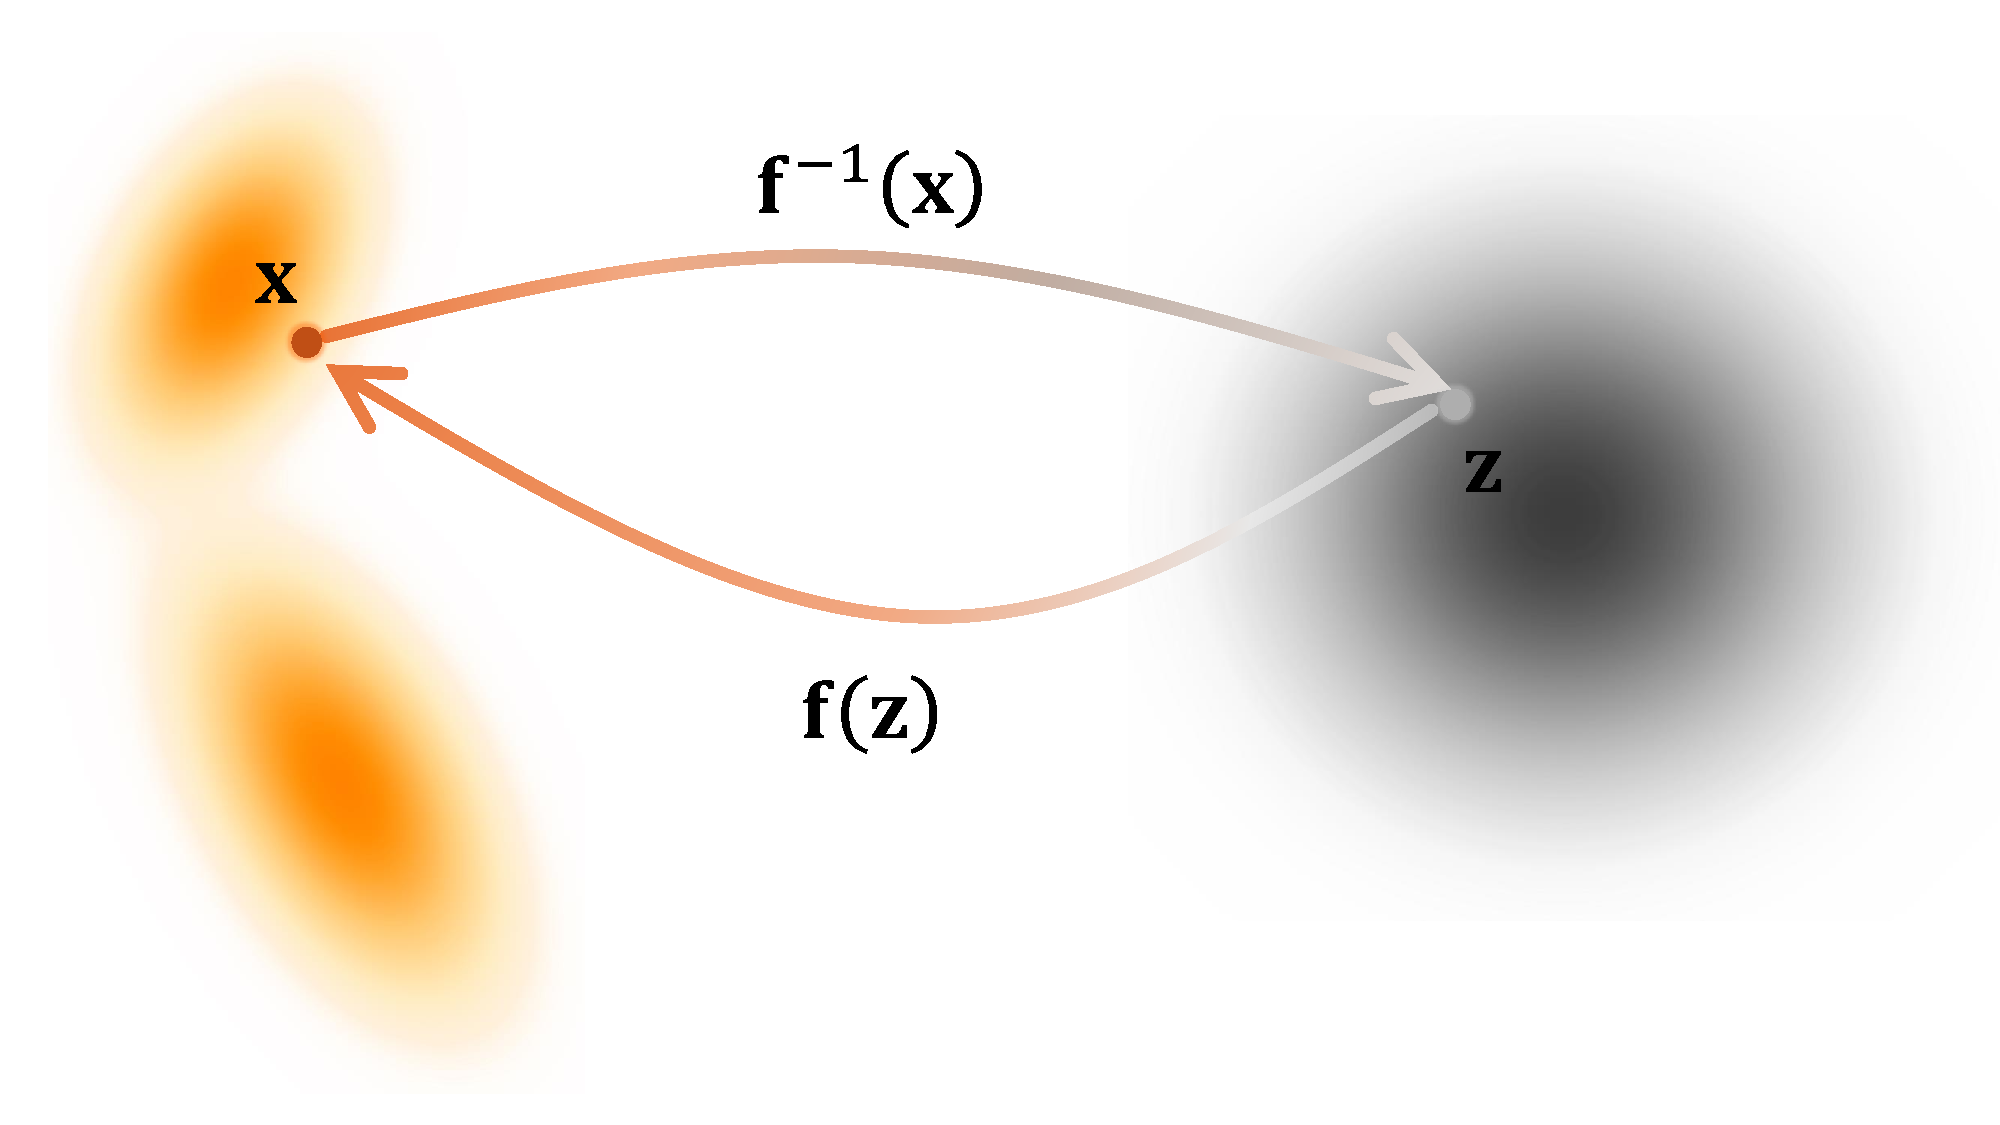
\includegraphics[width=0.76\linewidth]{Images/PartB/flow_density.pdf}
    \caption{\textbfs{Illustration of sample movement of NF under an invertible map.} It consists of a sequence of invertible functions $\rvf: \rvz \mapsto \rvx$ that transform latent variable $\rvz$ into a data $\rvx$, together with the inverse mapping $\rvf^{-1}: \rvx \mapsto \rvz$ that reconstructs the data. An NF resembles an encoder--decoder structure, but with the encoder realized as a smooth invertible map and the decoder given exactly by its inverse.    The corresponding change in density can be computed via the change-of-variables formula, as given in \Cref{eq:nf-change-of-var}. \figcredit{Created by the authors.}}
    \label{fig:sample-and-change-of-variable}
\end{figure}

\subsection{Normalizing Flows}

NFs~\citep{rezende2015variational} model a complex data distribution $p_{\text{data}}(\rvx)$ by transforming a simple prior $p_{\text{prior}}(\rvz)$ (e.g., standard Gaussian $\mathcal{N}(\bm{0}, \rmI)$) via an invertible mapping
\[
\rvf_{\bm{\phi}}: \mathbb{R}^D \to \mathbb{R}^D,
\]
with $\rvx = \rvf_{\bm{\phi}}(\rvz)$ and $\rvz \sim p_{\text{prior}}$. Here, $\rvx$ and $\rvz$ share the same dimension.
Using the change-of-variables formula in \Cref{eq:nf-change-of-var}, the model likelihood is\footnote{If the map is further constrained to be the gradient of a convex potential,
$\rvf_\bphi = \nabla \psi_\bphi$ with $\psi_\bphi$ convex, then
\Cref{eq:nf-change-of-var-log} reduces to the Monge--Ampère
relation in \Cref{eq:monge-ampere}.
This PDE characterizes the optimal transformation of one distribution into another under the quadratic cost. See \Cref{ch:ot-eot} and \citep{huangconvex} for further details.
}
\begin{align}\label{eq:nf-change-of-var-log}
\log p_{\bm{\phi}}(\rvx) = \log p_{\text{prior}}(\rvz) + \log \left| \det \frac{\partial \rvf_{\bm{\phi}}^{-1}(\rvx)}{\partial \rvx} \right|.
\end{align}




\paragraph{Training Objective.}
Parameters $\bm{\phi}$ are learned by maximizing the likelihood over data:
\begin{align}\label{eq:nf-training}
\mathcal{L}_{\text{NF}}(\bm{\phi}) = \mathbb{E}_{\rvx \sim p_{\text{data}}} \left[ \log p_{\bm{\phi}}(\rvx) \right].
\end{align}
Computing the Jacobian determinant in \Cref{eq:nf-change-of-var-log} can be costly, scaling as $\mathcal{O}(D^3)$ in general.

\paragraph{Constructing Invertible Transformations.}






A single complex invertible network can be expensive due to its Jacobian determinant. Conversely, simple transforms (e.g., linear) are efficient but lack expressivity.


To balance this, NFs employ a sequence of $L$ trainable invertible mappings $\{\rvf_k\}_{k=0}^{L-1}$, each with efficiently computable Jacobians:
\[
\rvf_{\bm{\phi}} = \rvf_{L-1} \circ \rvf_{L-2} \circ \cdots \circ \rvf_0.
\]
Each $\rvf_k$ is parameterized by a neural network, though we omit the explicit dependence on ${\bm{\phi}}$ for notational simplicity.


Samples transform via
\begin{align}\label{eq:nf-seq}
\rvx_{k+1} = \rvf_k(\rvx_k), \quad k = 0, \ldots, L-1,
\end{align}
with $\rvz=\rvx_0 \sim p_{\text{prior}}$ and $\rvx = \rvx_L$, corresponding to data. The resulting (log-)density is derived as 
\begin{align}\label{eq:multi-nf-density}
\begin{aligned}
    p_{\bm{\phi}}(\rvx) &= p_{\text{prior}}(\rvx_0) \prod_{k=0}^{L-1} \left| \det \frac{\partial \rvf_k}{\partial \rvx_k} \right|^{-1}, \text{ or equivalently,}\\
\log p_{\bm{\phi}}(\rvx) &= \log p_{\text{prior}}(\rvx_0) + \sum_{k=0}^{L-1} \log \left| \det \frac{\partial \rvf_k}{\partial \rvx_k} \right|^{-1}.
\end{aligned}
\end{align}


\vspace{0.3cm}
\begin{figure}[tbh!]
    \centering
\begin{tikzpicture}[
    ->, % Sets default arrow type
    >=Stealth, % Sets default arrowhead style
    node_dist/.style={left=1.7cm of #1}, % Position nodes to the LEFT
    font=\small,
    thick
  ]

  % Define a style for the nodes
  \tikzset{state/.style={
      rectangle,
      rounded corners=3pt,
      draw=black,
      fill=gray!10,
      minimum height=35pt,
      minimum width=25pt
    }
  }

  % Place the nodes from RIGHT to LEFT
  \node[state] (x0) {$\rvx_0 $};
  \node[state] (x1) [node_dist=x0] {$\rvx_1$};
  \node[state] (x2) [node_dist=x1] {$\rvx_2$};
  \node (dots) [left=0.7cm of x2] {$\boldsymbol{\cdots}$};
  \node[state] (xL) [node_dist=dots] {$\rvx_L$};

  % Draw the arrows (edges) with labels
  
  % Top path (Generative, right to left) - Shifted up
  \path [black] ([yshift=4.5pt]x0.west)  edge node[above] {$\rvf_0$} ([yshift=4.5pt]x1.east);
  \path [black] ([yshift=4.5pt]x1.west) edge node[above] {$\rvf_1$} ([yshift=4.5pt]x2.east);
  \path [black] ([yshift=4.5pt]x2.west) edge ([yshift=4.5pt]dots.east);
  \path [black] ([yshift=4.5pt]dots.west) edge node[above, pos=0.4] {$\rvf_{L-1}$} ([yshift=4.5pt]xL.east);
  
  % Bottom path (Inference, left to right) - Shifted down
  \path ([yshift=-4.5pt]x1.east) edge node[below] {$\rvf_0^{-1}$} ([yshift=-4.5pt]x0.west);
  \path ([yshift=-4.5pt]x2.east) edge node[below] {$\rvf_1^{-1}$} ([yshift=-4.5pt]x1.west);
  \path ([yshift=-4.5pt]dots.east) edge ([yshift=-4.5pt]x2.west);
  \path ([yshift=-4.5pt]xL.east) edge node[below, pos=0.6] {$\rvf_{L-1}^{-1}$} ([yshift=-4.5pt]dots.west);

\end{tikzpicture}
\caption{\textbfs{Illustration of a NF.} An NF consists of a stack of invertible maps
$\rvf_{\bm{\phi}} = \rvf_{L-1} \circ \rvf_{L-2} \circ \cdots \circ \rvf_0$. 
The transformation maps latent samples $\rvx_0 \sim p_{\mathrm{prior}}$ to data samples $\rvx_L \sim p_{\mathrm{data}}$. \figcredit{Created by the authors.}}
    \label{fig:nf-stack}
\end{figure}

\paragraph{Examples of Invertible Flows.} Extensive literature has focused on designing single-layer flow constructions that enable efficient computation of the Jacobian. Below, we introduce two representative types: Planar Flows~\citep{rezende2015variational} and Residual Flows~\citep{chen2019residual,behrmann2019invertible}, with the latter motivating the developments in \Cref{subsec:NODE}.
\subparagraph{Planar Flows:}
Planar flows~\citep{rezende2015variational} apply a simple transformation
\[
\rvf(\rvz)
=
\rvz
+
\rvu h(\rvw^\top\rvz+b),
\]
where $\rvu,\rvw\in\mathbb{R}^D$, $b\in\mathbb{R}$, and $h(\cdot)$ is an
activation function. The parameters are appropriately constrained or
reparameterized to ensure that the transformation is invertible. Its Jacobian
determinant has the simple form
\[
\left|
\det\frac{\partial\rvf(\rvz)}{\partial\rvz}
\right|
=
\left|
1+h'(\rvw^\top\rvz+b)\,\rvw^\top\rvu
\right|,
\]
making the change-of-variables computation efficient.

\subparagraph{Residual Flows:}
Define the transform $\rvf$ as
\begin{align}\label{eq:residual-flow}
\rvf(\rvz) = \rvz + \rvv(\rvz),
\end{align}
with $\rvv$ contractive (Lipschitz constant $< 1$). This ensures invertibility via the Banach fixed-point theorem.

The log-determinant of the Jacobian reduces to a trace expansion:
\begin{align}\label{eq:log-det-tr}
    \log \Bigg|\det \frac{\partial \rvf(\rvz)}{\partial \rvz} \Bigg| &= \log \left( \det \frac{\partial \rvf(\rvz)}{\partial \rvz} \right) \nonumber\\
    &= \Tr\left(\log\left(\frac{\partial \rvf(\rvz)}{\partial \rvz}\right)\right) \nonumber\\
    &= \Tr\left(\log\left(\rmI + \frac{\partial \rvv(\rvz)}{\partial \rvz}\right)\right) \nonumber\\
    &= \sum_{k=1}^{\infty} \frac{(-1)^{k+1}}{k} \Tr\left(\left(\frac{\partial \rvv(\rvz)}{\partial \rvz}\right)^k\right),
\end{align}
making evaluation efficient via trace estimators~\citep{hutchinson1989stochastic}.

\paragraph{Sampling and Inference.}
Sampling from NFs is straightforward: draw $\rvx_0 \sim p_{\text{prior}}$ and compute $\rvx = \rvf_{\bm{\phi}}(\rvx_0)$. Exact likelihoods are obtained from \Cref{eq:multi-nf-density}.


\subsection{Neural ODEs}\label{subsec:NODE}
\begin{figure}[th!]
    \centering
    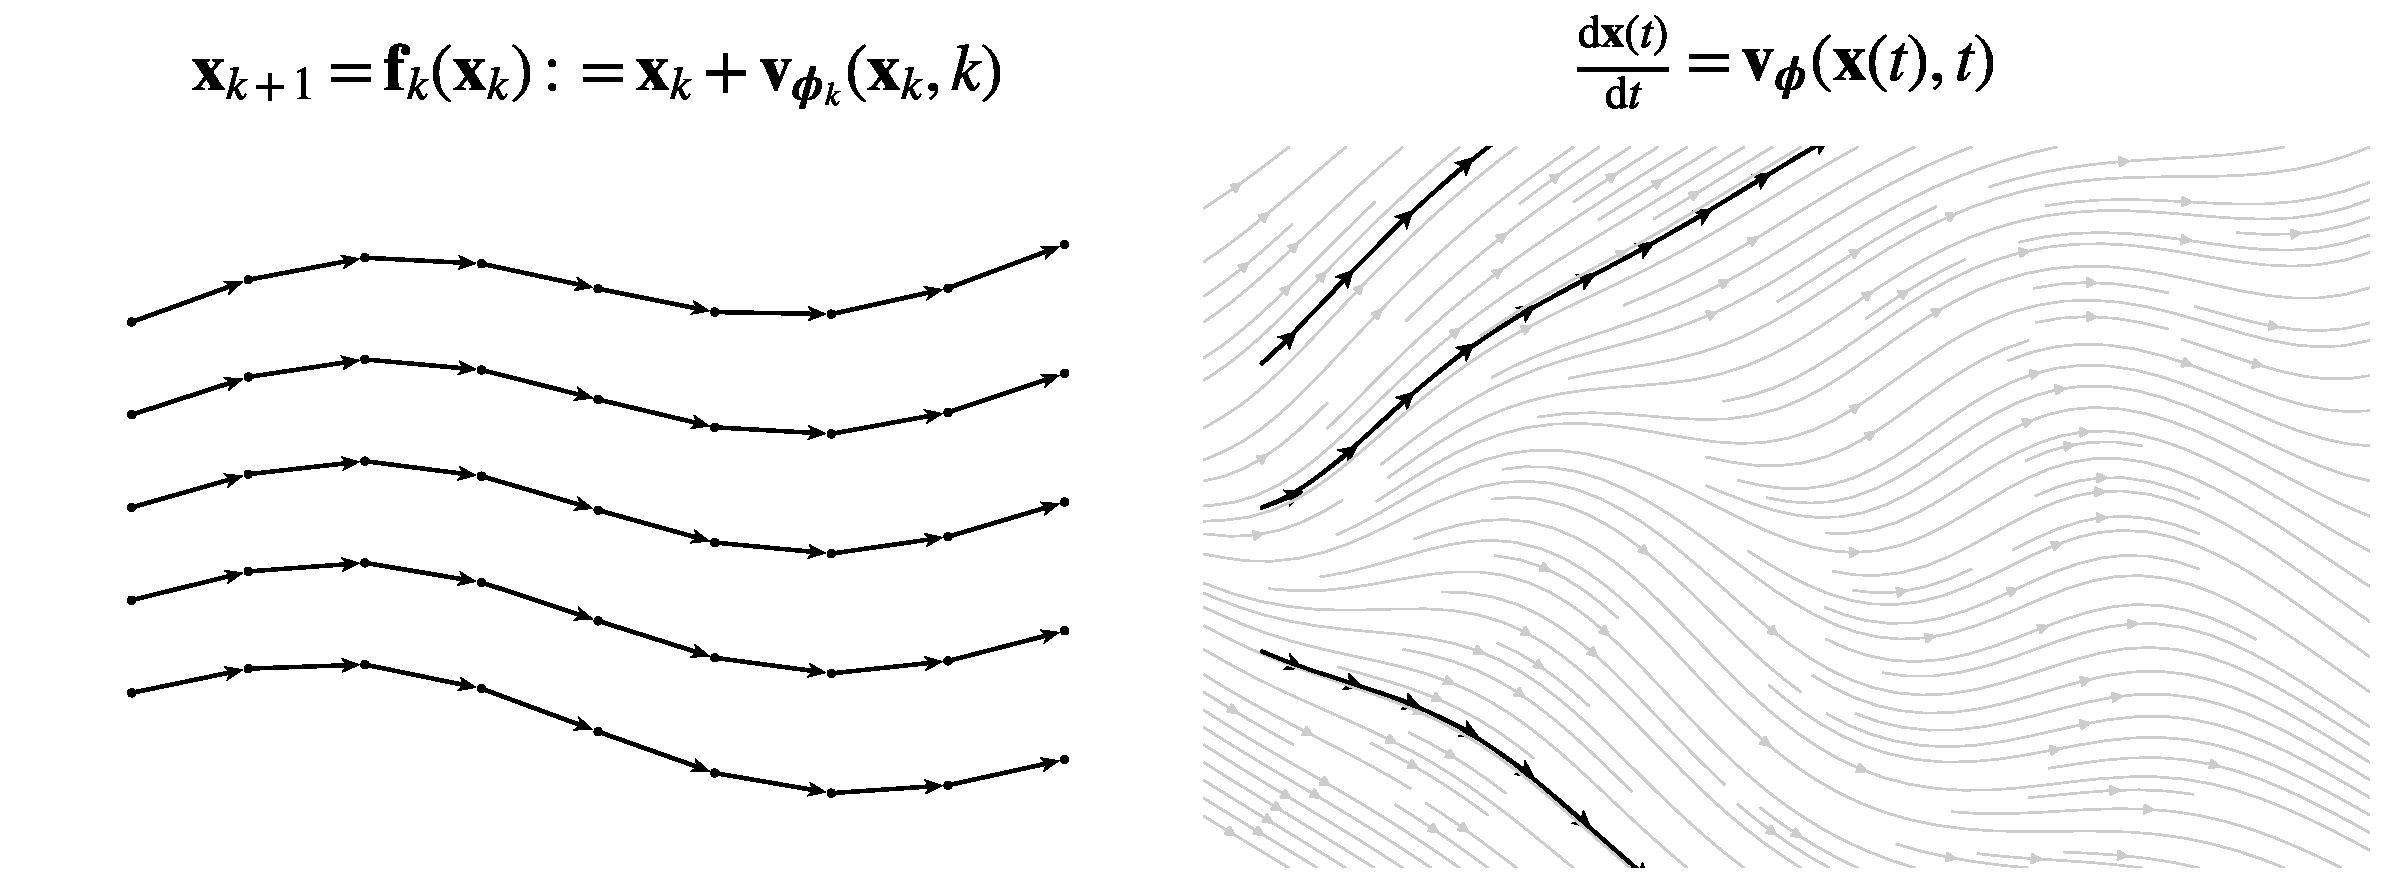
\includegraphics[width=\linewidth]{Images/PartB/discrete_vs_continuous_side_by_side_white.pdf}
    \caption{\textbfs{Discrete- vs. continuous-time normalizing flows.} (Left) A discrete NF transports samples by a finite sequence of invertible maps  $\mathbf{x}_{k+1} = \mathbf{f}_k(\mathbf{x}_k)$,
yielding stepwise, non-crossing trajectories (dots with arrows). (Right) A continuous NF (Neural ODE) evolves states along integral curves of $\frac{\diff\mathbf{x}(t)}{\diff t} = \mathbf{v}_{\boldsymbol{\phi}}(\mathbf{x}(t),t)$,
where black paths with tangent arrows are shown over the gray vector field. \figcredit{Created by the authors.}}
    \label{fig:nf-cnf}
\end{figure}


% \paragraph{From Discrete-Time NFs to Continuous-Time NFs (Neural ODEs).} 
% NFs are typically formulated as a sequence of $L$ discrete, invertible transformations. Viewed through the lens of \Cref{eq:nf-seq} and the ``Residual Flow'' formulation in \Cref{eq:residual-flow}, each layer can be written as the following:
% \[
% \rvx_{k+1} = \rvf_k(\rvx_k) := \rvx_k + \rvv_{\bm{\phi}_k}(\rvx_k, k),
% \]
% where $\rvv_{\bm{\phi}_k}(\cdot, k)$ is a layer-dependent velocity field parameterized by neural networks. Intuitively, this velocity field is a learned vector-valued function that ``pushes'' the data points in the input space in small, smooth steps. Each transformation moves points along the directions suggested by this velocity, gradually morphing the simple  prior distribution into the complex target distribution. 


% This formulation, indeed, corresponds to the Euler discretization of the continuous-time ODE with learnable parameter $\bphi$:
% \[
% \frac{\diff \rvx(t)}{\diff t} = \rvv_{\bm{\phi}}(\rvx(t), t).
% \]
%  In the limit of infinite layers and vanishing step size ($\Delta t \to 0$), the discrete NFs converges to a continuous model, yielding the framework of \emph{Neural ODEs} (NODEs)~\citep{chen2018neural}, also known as \emph{Continuous Normalizing Flows} (CNFs).

\paragraph{From Discrete-Time NFs to Continuous-Time NFs (Neural ODEs).}
A discrete NF transports samples through a composition of $L$ invertible
maps. To obtain a meaningful continuous-depth limit, we write each layer
as a small residual update:
\[
\rvx_{k+1}
=
\rvx_k+\Delta t\,\rvv_{\bm{\phi}}(\rvx_k,t_k),
\qquad
t_k=k\Delta t,
\qquad
\Delta t=\frac{T}{L}.
\]
Here, $\rvv_{\bm{\phi}}$ specifies the direction in which each point is
moved, while $\Delta t$ controls the size of one layer.

The geometric meaning of this limit is illustrated in
\Cref{fig:bijection-continuity}. As $L$ increases, the same
source-to-target transport is divided into more near-identity bijections.
The sample trajectories are resolved more finely, and the deformation of
the surrounding reference grid becomes progressively smoother.

As $L\rightarrow\infty$ and $\Delta t\rightarrow 0$, the discrete layer
index becomes continuous time, yielding the ODE
\[
\frac{\diff \rvx(t)}{\diff t}
=
\rvv_{\bm{\phi}}(\rvx(t),t).
\]
This continuous-depth model is known as a Neural ODE or Continuous
Normalizing Flow.



\begin{figure}[th!]
    \centering
    
\includegraphics[width=\linewidth]{Images/PartB/cov_2d_layers.pdf}
    \caption{\textbfs{From discrete bijections to a continuous transport flow.}
    Each panel shows a transport built by composing $L$ invertible layers.
    Starting from a source distribution (Gaussian), the layers gradually move
    the colored samples toward a target distribution with three modes. The
    orange reference grid shows how the surrounding space is deformed during
    this transport. With only a few layers, each layer makes a relatively
    large and discrete change. As $L$ increases, the transport is divided
    into more, smaller updates, so the sample trajectories and grid
    deformation become smoother. If the total transport time $T$ is fixed
    and each layer has step size $\Delta t=T/L$, then, as
    $L\rightarrow\infty$, the stacked bijections approach a continuous
    time-dependent flow. The transported density evolves according to the
    continuity equation in \Cref{eq:continuity_eq}.
    \figcredit{Created by the authors with AI-assisted coding.}}
    \label{fig:bijection-continuity}
\end{figure}


\paragraph{Formal Setup of Neural ODEs.}
A Neural ODE defines a continuous transformation through:
\begin{align}\label{eq:neural-ode}
    \frac{\diff \rvx(t)}{\diff t} = \rvv_{\bm{\phi}}(\rvx(t), t),\quad t\in [0,T]
\end{align}
where:
\begin{itemize}
    \item $ \rvx(t) \in \mathbb{R}^D $ is the state at time $t$; we sometimes write $\rvx_t$ for brevity;
    \item $\rvv_{\bm{\phi}}(\rvx(t), t)$ is a neural network parameterized by $\bm{\phi}$.
\end{itemize}


\subparagraph{Goal of NODE.}
Starting from the initial condition $\rvx(0) \sim p_{\text{prior}}$, the ODE evolves the state continuously over time, inducing a family of marginal distributions $p_{\bm{\phi}}(\rvx_t, t)$ (similar to PF-ODEs!)\footnote{We adopt a flipped time convention, with $t = 0$ denoting the prior (source) and $t = 1$ the data (target) distribution. The prior is interchangeably written as $p_{\bm{\phi}}(\rvx(0), 0)$, $p_{\text{prior}}(\rvx(0), 0)$, or simply $p_{\text{prior}}(\rvz)$.
}. 

The goal is to learn the neural vector field $\rvv_{\bm{\phi}}$, which intuitively represents a velocity that transports points along continuous trajectories in data space. By learning this velocity, the terminal distribution at $t=T$ matches the target distribution $p_{\mathrm{data}}(\cdot)$. This continuous transformation unifies discrete normalizing flows and neural ODEs within a single framework.



\paragraph{Continuous-Time Change-of-Variables Formula.}
Analogous to \Cref{eq:nf-change-of-var} or \Cref{eq:multi-nf-density},
\citet{chen2018neural} derived a continuous-time analogue of the
change-of-variables formula. For the time-dependent density
$p_{\bm{\phi}}(\rvx(t),t)$ of a process $\rvx(t)$ evolving under
\Cref{eq:neural-ode}, the so-called \emph{Instantaneous
Change-of-Variables Formula} is
\[
\frac{\diff}{\diff t}
\log p_{\bm{\phi}}(\rvx(t),t)
=
-\nabla_{\rvx}\cdot
\rvv_{\bm{\phi}}(\rvx(t),t).
\]
Here, the derivative is taken along the ODE trajectory $\rvx(t)$.

Therefore, if $\rvx(0)\sim p_{\mathrm{prior}}$ and the ODE transports the
prior from $t=0$ to $t=T$, integrating this identity gives
\begin{align}\label{eq:NODE-likelihood}
\log p_{\bm{\phi}}(\rvx(T),T)
=
\log p_{\mathrm{prior}}(\rvx(0))
-
\int_0^T
\nabla_{\rvx}\cdot
\rvv_{\bm{\phi}}(\rvx(t),t)
\,\diff t.
\end{align}
This expression provides likelihood evaluation through numerical integration,
which in turn enables maximum likelihood training of the model.

Although this formula may appear unfamiliar at first, it is closely connected
to the Fokker--Planck equation. In particular, it can be understood as the
along-trajectory form of the \emph{continuity equation}, which is the
deterministic, zero-diffusion case of the Fokker--Planck equation
(see \Cref{app:continuity}). It can also be interpreted as the continuous-time
limit of the discrete change-of-variables formula in
\Cref{eq:multi-nf-density}. We summarize the result below.

\lemp{Instantaneous Change of Variables}{instant-change-of-var}{
Let $\rvz(t)$ be a continuous random process with time-dependent density
$p(\rvz(t),t)$, and suppose it evolves according to the ODE
\begin{align*}
\frac{\diff\rvz(t)}{\diff t}
=
\mathbf{F}(\rvz(t),t).
\end{align*}
Assuming sufficient regularity so that the ODE flow and the evolving density
are well defined, the log-density along the trajectory satisfies
\begin{align}\label{eq:instant-change-of-var}
\frac{\diff}{\diff t}
\log p(\rvz(t),t)
=
-\nabla_{\rvz}\cdot
\mathbf{F}(\rvz(t),t).
\end{align}
}{
This follows from the continuity equation together with the chain rule. We present detailed alternative derivations in \Cref{app-sec:flow-proof}.}


\subparagraph{Connection to Discrete-Time Formula.}  
The NODE likelihood in \Cref{eq:NODE-likelihood},
\[
\log p_{\bm{\phi}}(\rvx(T), T) = \log p_{\text{prior}}(\rvx(0), 0) - \int_0^T \nabla_\rvx \cdot \rvv_{\bm{\phi}}(\rvx(t), t) \diff t,
\]
can be seen as the continuous-time analogue of the discrete normalizing flow formulation in \Cref{eq:multi-nf-density}:
\[
\log p_{\bm{\phi}}(\rvx_L) = \log p_{\text{prior}}(\rvx_0) - \sum_{k=0}^{L-1} \log \left| \det \frac{\partial \rvf_k}{\partial \rvx_k} \right|.
\]
The integral mirrors the summation, and the trace operator replaces the log-determinant, as discussed in \Cref{eq:log-det-tr}. These parallels are further explored in the proof of the lemma.

\paragraph{Training NODEs.}  
Based on \Cref{eq:NODE-likelihood}, NODEs learn a parameterized velocity field $\rvv_{\bm{\phi}}$ such that the terminal distribution
\[
p_{\bm{\phi}}(\cdot, T) \approx p_{\text{data}},
\]
where trajectories evolve from latent variables $\rvx(0) \sim p_{\text{prior}}$ via the ODE flow. Training follows the MLE framework from \Cref{eq:MLE}:
\[
\mathcal{L}_{\text{NODE}}(\bm{\phi}) := \mathbb{E}_{\rvx \sim p_{\text{data}}} \big[\log p_{\bm{\phi}}(\rvx, T)\big].
\]

\subparagraph{Exact Log-Likelihood Computation.} 
To compute $\log p_{\bm{\phi}}(\mathbf{x}, T)$ for data point $\mathbf{x}$, we integrate the change-of-variables formula \eqref{eq:NODE-likelihood}:
\begin{align}
\log p_{\bm{\phi}}(\mathbf{x}, T) = \log p_{\text{prior}}(\mathbf{z}(0)) - \int_0^T \nabla_{\mathbf{z}} \cdot \mathbf{v}_{\bm{\phi}}(\mathbf{z}(t), t) \diff t.
\end{align}
Here, $\mathbf{z}(t)$ solves the ODE reversely from $t = T$ to $t = 0$:
\[
\frac{\diff\mathbf{z}(t)}{\diff t} = \mathbf{v}_{\bm{\phi}}(\mathbf{z}(t), t)
\]
with $\mathbf{z}(T) = \mathbf{x}$. The prior term $\log p_{\text{prior}}(\mathbf{z}(0))$ is tractable for standard distributions. This enables exact likelihood-based training and evaluation in neural ODEs.

\subparagraph{Gradient-Based Optimization.}  
Maximizing $\mathcal{L}_{\text{NODE}}$ requires backpropagation through the ODE solver. The adjoint sensitivity method~\citep{pontryagin2018mathematical, chen2018neural} computes gradients via an auxiliary ODE with $\mathcal{O}(1)$ memory complexity, but NODE training remains expensive due to numerical integration at each step.

\paragraph{Inference with NODEs.}  
Sampling with a trained model $\rvv_{\bm{\phi}^\times}$ proceeds by drawing $\rvx(0) \sim p_{\text{prior}}$ and integrating forward (by numerical solvers):
\[
\rvx(T) = \rvx(0) + \int_0^T \rvv_{\bm{\phi}^\times}(\rvx(t), t)   \diff t.
\]
The terminal state $\rvx(T)$ approximates a sample from $p_{\text{data}}$.

Moreover, we note that for any vector field $\rmF$, the following identity holds:
\[
    \Tr\left(\frac{\partial \rmF}{\partial \rvz(t)} \right) = \nabla_{\rvz} \cdot \rmF.
\]
Hence, the divergence can be estimated efficiently using stochastic trace
estimators, such as Hutchinson's estimator~\citep{hutchinson1989stochastic},
without explicitly constructing the full Jacobian. This makes likelihood
evaluation much more practical in high-dimensional settings. However, because
the trace is then estimated from random samples, the resulting numerical
log-likelihood estimate is stochastic rather than an exact evaluation of the
divergence.

Having seen in \Cref{fig:bijection-continuity} how many small bijections
approach a continuous transport flow, we now ask a practical question:
\begin{question}
    How can we learn its velocity field without repeatedly solving an ODE
during training?
\end{question}
 This question leads naturally to Flow Matching, which
learns the velocity field directly through a simulation-free regression
objective and provides the flow-based perspective on diffusion models.
% \subsection{Closing Remarks}\label{subsec:remark-flow}
%  We first compare NODEs with discrete NFs, then outline their connection to diffusion models.
% \paragraph{Advantages of NODEs over Discrete NFs.}
% NODEs offer two key advantages:
% \begin{enumerate}
%     \item \textbfs{Flexible Architectures:} Unlike discrete NFs, NODEs do not require invertible transformations, as ODE solutions are guaranteed under Lipschitz conditions on the velocity field $\rvv_{\bm{\phi}}$.
%     \item \textbfs{Efficient Likelihoods Computation:} NODEs compute divergence $\nabla \cdot \rvv_{\bm{\phi}}$ with $\mathcal{O}(D)$ complexity, compared to the $\mathcal{O}(D^3)$ Jacobian determinant in discrete NFs, enabling high-dimensional scalability.
% \end{enumerate}
% Beyond generative modeling, NODEs are also used in dynamical systems, time series, and mathematical physics~\citep{kidger2022neural}.


% \paragraph{What Lies Ahead?}
% In this section, we have examined the development of NFs and NODEs:
% \begin{itemize}
%     \item \textbfs{Stage 1.} Single-layer invertible transformations in NFs;
%     \item \textbfs{Stage 2.} Multiple layers of invertible transformations in NFs;
%     \item \textbfs{Stage 3.} Continuous-time extension through NODEs, equivalent to infinitely many layers of invertible transformations.
% \end{itemize}

% It is fascinating to see how the evolution of flow-based models echoes that of VAEs~(\Cref{ch:variational}) and score-based methods~(\Cref{ch:score-based}). Each of these modeling paradigms embarks on a similar journey: beginning with simple, discrete-time, single-layer structures, advancing to deeper multi-layer designs (e.g., DDPM/NCSN), and ultimately converging toward elegant continuous-time formulations (Score SDE).

% However, a crucial difference emerges: even though diffusion models are associated with an ODE (i.e., PF-ODE), they do not directly learn an arbitrary velocity field $\mathbf{v}_{\bm{\phi}}$ as in NODEs. Instead, diffusion models learn objectives (e.g., score) that define ODEs aimed at matching prescribed marginal distributions--governed by Fokker-Planck equation. This approach makes diffusion model training simulation-free and thus computationally efficient, in contrast to NODEs which require solving numerical ODEs during training.

% Flow matching inherits this essential characteristic of diffusion model training and resolves the simulation bottleneck of NODEs, enabling efficient distribution-to-distribution transport via ODEs with prescribed underlying structure. We will explore this further in the next chapter.




\newpage
\clearpage
\section{\texorpdfstring{Flow Matching Framework}{Flow Matching Framework}}\label{sec:flow-matching-framework}

Both Score SDEs~(\Cref{ch:score-sde}) and
NODEs~(\Cref{sec:flow-based-method}) describe generative modeling as a
continuous transport process. Score SDEs formulate this transport through
stochastic dynamics together with an associated PF-ODE,
whereas NODEs directly parameterize a deterministic ODE. In the standard
generative setting, both aim to transport a simple Gaussian prior
$p_{\mathrm{prior}}$ into the data distribution $p_{\mathrm{data}}$.

A practical limitation of NODEs is that likelihood-based training requires
repeatedly solving an ODE. The \emph{Flow Matching} (FM)
framework~\citep{lipman2022flow,lipman2024flow,tongimproving} avoids this
cost by training a neural network to predict the velocity field directly
through a regression objective. ODE integration is therefore needed for
generation, but not inside the training loop, making FM training
simulation-free.

More generally, FM is not restricted to Gaussian-to-data transport. It
considers a source distribution $p_{\mathrm{src}}$ and a target
distribution $p_{\mathrm{tgt}}$, both assumed to be easy to sample from.
Standard generative modeling is recovered as the special case
\[
p_{\mathrm{src}}=p_{\mathrm{prior}},
\qquad
p_{\mathrm{tgt}}=p_{\mathrm{data}},
\]
where $p_{\mathrm{prior}}$ is typically Gaussian.

In this section, we adopt the FM viewpoint\footnote{Several related
approaches share the core idea of transporting between endpoint
distributions using a continuous-time flow, although their formulations
differ slightly. These include Flow Matching
(FM)~\citep{lipman2022flow,neklyudov2023action}, Rectified Flow
(RF)~\citep{liu2022rectified,heitz2023iterative}, and Stochastic
Interpolants~\citep{albergo2023stochastic,albergobuilding,ma2024sit}.
Here, we use FM as a unifying terminology.}
Its goal is to learn a time-dependent velocity field
$\mathbf{v}_t(\rvx_t)$ whose associated ODE transports samples along a
prescribed probability path $\{p_t\}_{t\in[0,1]}$ satisfying
\[
p_0=p_{\mathrm{src}},
\qquad
p_1=p_{\mathrm{tgt}}.
\]
When $p_{\mathrm{src}}$ is Gaussian, we refer to this setting as
\emph{Gaussian Flow Matching}. Thus, FM provides both a simulation-free
training method for generative modeling and a general framework for
learning continuous transport between arbitrary endpoint distributions.

% Both Score SDEs~(\Cref{ch:score-sde}) and
% NODEs~(\Cref{sec:flow-based-method}) describe generative modeling as a
% continuous transport process. Score SDEs use stochastic dynamics, together
% with an associated probability-flow ODE, while NODEs directly parameterize
% a deterministic ODE. In either case, the goal is to transport a simple
% Gaussian prior sample
% $\bm{\epsilon}\sim p_{\mathrm{prior}}$
% into a data-like sample from $p_{\mathrm{data}}$.

% The \emph{Flow Matching} (FM) framework
% ~\citep{lipman2022flow,lipman2024flow,tongimproving} builds on this
% continuous-transport viewpoint and generalizes it beyond the usual
% Gaussian-to-data setting. It considers two arbitrary endpoint
% distributions: a source distribution $p_{\mathrm{src}}$ and a target
% distribution $p_{\mathrm{tgt}}$, both of which are assumed to be easy to
% sample from. Standard generative modeling is recovered as the special case
% in which $p_{\mathrm{src}}$ is a Gaussian prior and
% $p_{\mathrm{tgt}}=p_{\mathrm{data}}$.

% In this section, we adopt the FM viewpoint\footnote{Several related
% approaches share the core idea of transporting between endpoint
% distributions using a continuous-time flow, although their formulations
% differ slightly. These include Flow Matching
% (FM)~\citep{lipman2022flow,neklyudov2023action}, Rectified Flow
% (RF)~\citep{liu2022rectified,heitz2023iterative}, and Stochastic
% Interpolants~\citep{albergo2023stochastic,albergobuilding,ma2024sit}.
% Here, we use FM as a unifying terminology.}
% Its central goal is to learn a time-dependent velocity field
% $\mathbf{v}_t(\rvx_t)$ whose associated ODE transports samples along a
% prescribed probability path $\{p_t\}_{t\in[0,1]}$ satisfying
% \[
% p_0=p_{\mathrm{src}},
% \qquad
% p_1=p_{\mathrm{tgt}}.
% \]
% When $p_{\mathrm{src}}$ is Gaussian, we refer to this setting as
% \emph{Gaussian Flow Matching}. Like diffusion models, FM permits
% simulation-free training; more generally, it provides a flexible framework
% for learning continuous transport between arbitrary distributions using
% only samples from the endpoints.



\subsection{Lesson from Score-Based Methods}\label{subsec:lesson-score}

We revisit the Score SDE framework (\Cref{ch:score-sde}) using a slightly different but equivalent formulation to extract key insights that motivate the FM approach. This analysis reveals how diffusion models implicitly learn probability flows and motivates a more direct formulation.


\paragraph{Step 1: Defining a Conditional Path and Its Marginal Densities.}

\begin{figure}[th!]
    \centering
    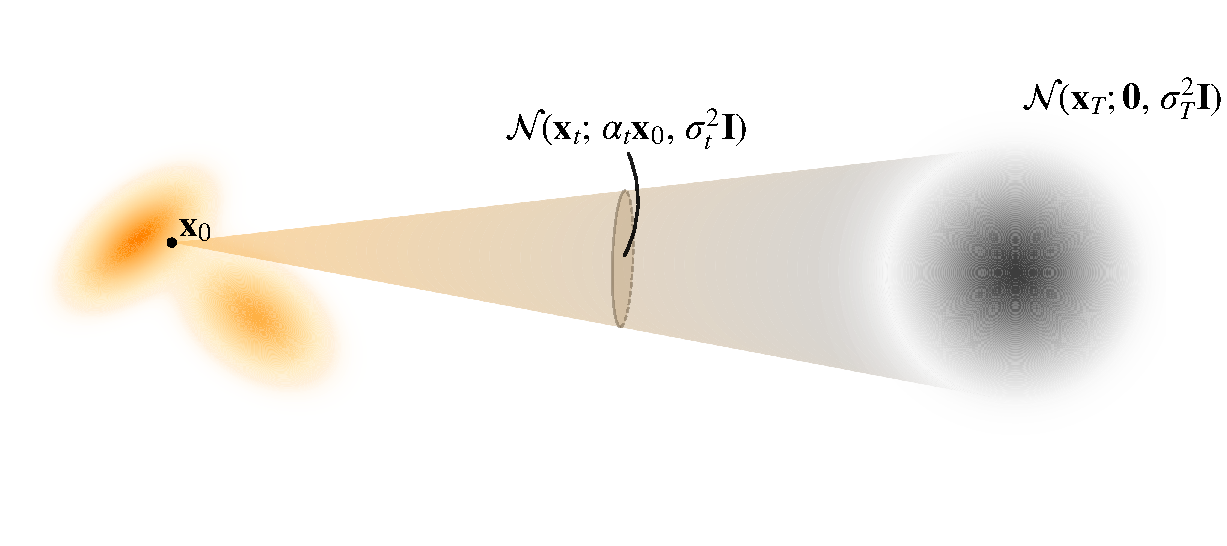
\includegraphics[width=\linewidth]{Images/PartB/data_vs_prior_cone_with_oval.pdf}
    % \vspace{-1.5cm}
    \caption{\textbfs{Illustration of the conditional transition distribution.} 
$p_t(\rvx_t | \rvx_0) = \mathcal{N}(\rvx_t;\alpha_t \rvx_0,\sigma_t^2 \mathbf{I})$, 
defines a (Gaussian) conditional probability path from a data sample 
$\rvx_0 \sim p_{\text{data}}$ (left) towards the Gaussian prior 
$p_{\text{prior}}$ (right). \figcredit{Created by the authors.}}
    \label{fig:data-prior-conditioning}
\end{figure}

A diffusion model specifies a continuous-time family of densities $\{p_t\}_{t \in [0,1]}$ that transports a simple prior $p_{\text{prior}}$ (e.g., Gaussian) at $t=1$, used as the source, to a target data distribution $p_{\text{data}}$ at $t=0$:
\[
p_1(\rvx_1) = p_{\text{prior}}(\rvx_1), \quad p_0(\rvx_0) = p_{\text{data}}(\rvx_0).
\]
This path is implicitly defined via the forward conditional distribution
\begin{align}\label{eq:lesson-dm-conditional-path}
    p_t(\rvx_t|\rvx_0) = \mathcal{N}(\rvx_t; \alpha_t \rvx_0, \sigma_t^2 \mathbf{I}), \quad \rvx_0\sim p_{\text{data}}
\end{align}
which induces the marginal density
\[
p_t(\rvx_t) := \int p_t(\rvx_t |\rvx_0)  p_{\text{data}}(\rvx_0) \mathrm{d}\rvx_0.
\]
The increasing variance $\sigma_t^2$ of the conditional Gaussian drives the evolution of $p_t$ toward the Gaussian prior.

\paragraph{Step 2: Velocity Field.}
The time evolution of the marginal density $p_t$ is governed by a velocity field $\rvv_t : \mathbb{R}^D \to \mathbb{R}^D$, derived from the Fokker-Planck equation:
\begin{align}\label{eq:dm-velocity}
    \rvv_t(\rvx) := f(t)\rvx - \frac{1}{2}g^2(t)\nabla_{\rvx} \log p_t(\rvx),
\end{align}
which defines a deterministic particle flow through the PF-ODE:
\[
\frac{\diff \rvx(t)}{\diff t} = \underbrace{f(t)\rvx(t) - \frac{1}{2}g^2(t)\nabla_{\rvx} \log p_t\big(\rvx(t)\big)}_{\rvv_t(\rvx(t))}.
\]
This ODE transports an initial random variable $\rvx(0) \sim p_{\text{data}}$ forward in time or $\rvx(1) \sim p_{\text{prior}}$ backward in time, such that the evolving marginal density of $\rvx(t)$ matches $p_t$ at every $t \in [0,1]$  (see ``Underlying Rule'' below).

The scalar functions $f(t)$ and $g(t)$ are determined by the coefficients of the associated forward SDE, or equivalently the Gaussian kernel parameters $\alpha_t$ and $\sigma_t$ defined in the conditional path (see Lemma~\ref{forward-sde}).


\paragraph{Step 3: Learning via the Conditional Strategy.}
The PF-ODE velocity in \Cref{eq:dm-velocity} depends on the marginal score
$\nabla_{\rvx_t}\log p_t(\rvx_t)$, which is generally unknown.
Score-based methods therefore learn this score using a neural network
$\rvs_{\bm{\phi}}(\rvx_t,t)$ through the ideal score-matching objective
\[
\mathcal{L}_{\text{SM}}(\bm{\phi})
=
\mathbb{E}_{t\sim\mathcal{U}[0,1],\,\rvx_t\sim p_t}
\left[
\left\|
\rvs_{\bm{\phi}}(\rvx_t,t)
-
\nabla_{\rvx_t}\log p_t(\rvx_t)
\right\|^2
\right].
\]
Once the score is learned, the PF-ODE velocity is obtained from it as
\[
\rvv_t(\rvx_t)
=
f(t)\rvx_t
-
\frac{1}{2}g^2(t)
\nabla_{\rvx_t}\log p_t(\rvx_t),
\]
with $\rvs_{\bm{\phi}^\times}(\rvx,t) \approx \nabla_{\rvx_t}\log p_t(\rvx)$

The difficulty is that the marginal score itself is inaccessible when computing the regression target.
As in \Cref{ch:score-based}, we overcome this using the conditioning trick.
The conditional distribution $p_t(\rvx_t|\rvx_0)$ is tractable, and its
conditional score satisfies
\begin{align}\label{eq:marginal-oracle-score}
\nabla_{\rvx_t}\log p_t(\rvx_t)
=
\mathbb{E}_{\rvx_0\sim p(\cdot|\rvx_t)}
\left[
\nabla_{\rvx_t}\log p_t(\rvx_t|\rvx_0)
\right].
\end{align}
This motivates the denoising score matching objective
\[
\mathcal{L}_{\text{DSM}}(\bm{\phi})
:=
\mathbb{E}_{t,\,\rvx_0\sim p_{\mathrm{data}},\,
\rvx_t\sim p_t(\cdot|\rvx_0)}
\left[
\left\|
\rvs_{\bm{\phi}}(\rvx_t,t)
-
\nabla_{\rvx_t}\log p_t(\rvx_t|\rvx_0)
\right\|^2
\right].
\]
As shown in Theorem~\ref{thm:sm-dsm}, $\mathcal{L}_{\text{SM}}$ and
$\mathcal{L}_{\text{DSM}}$ differ only by a constant independent of
$\bm{\phi}$ and therefore have the same population minimizer:
\[
\rvs^*(\rvx_t,t)
=
\mathbb{E}_{\rvx_0\sim p(\cdot|\rvx_t)}
\left[
\nabla_{\rvx_t}\log p_t(\rvx_t|\rvx_0)
\right]
=
\nabla_{\rvx_t}\log p_t(\rvx_t).
\]

Importantly, the same conditioning principle can also be expressed directly
at the level of the PF-ODE velocity. Define the conditional velocity
\[
\rvv_t(\rvx_t|\rvx_0)
:=
f(t)\rvx_t
-
\frac{1}{2}g^2(t)
\nabla_{\rvx_t}\log p_t(\rvx_t|\rvx_0).
\]
Using \Cref{eq:marginal-oracle-score}, we immediately obtain
\[
\rvv_t(\rvx_t)
=
\mathbb{E}_{\rvx_0\sim p(\cdot|\rvx_t)}
\left[
\rvv_t(\rvx_t|\rvx_0)
\right].
\]
Thus, score-based diffusion learns the score through tractable conditional
targets and then uses it to construct the PF-ODE velocity. Flow Matching will
apply the same conditional-to-marginal principle directly to the velocity
field.
\begin{figure}
    \centering
    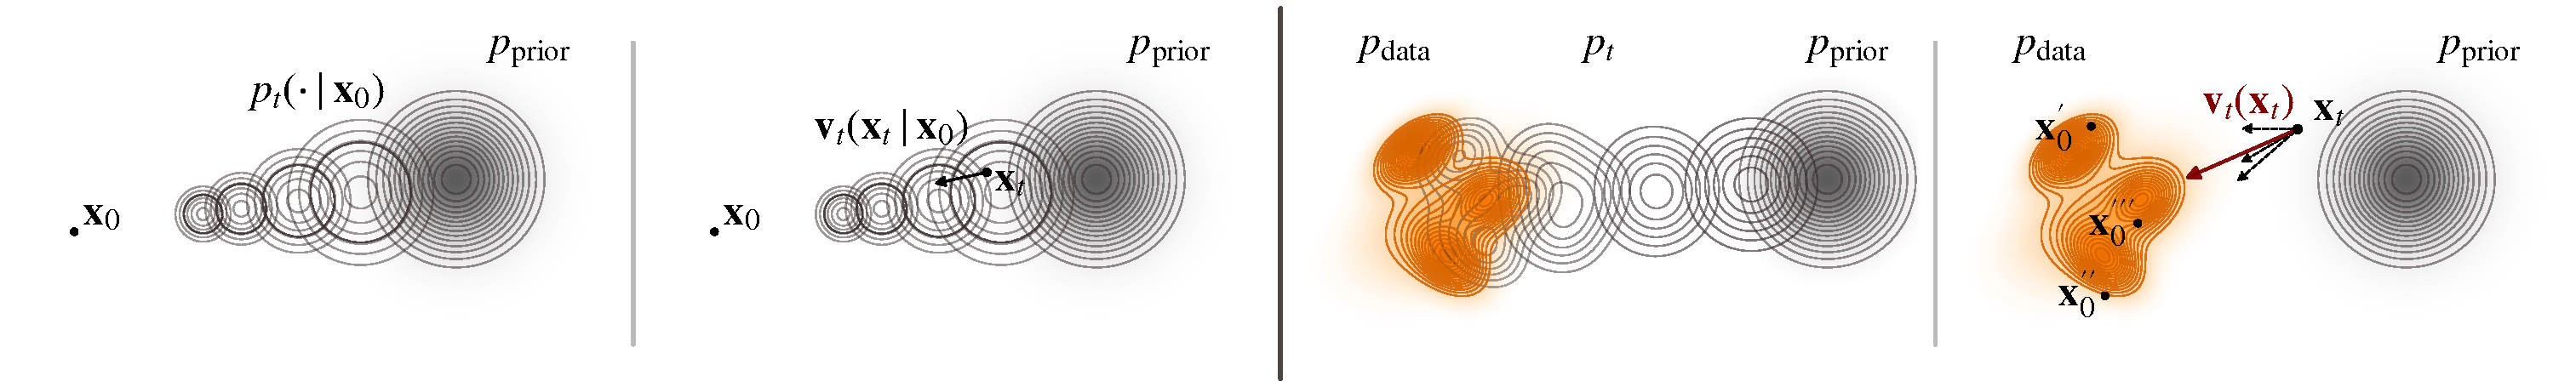
\includegraphics[width=\linewidth]{Images/PartB/four_panel_simple.pdf}
    \caption{\textbfs{Illustration of conditional versus marginal perspectives in diffusion.} (This figure is motivated by \citet{lipman2024flow}.) 
(1) Conditional Gaussian path $p_t(\cdot|\mathbf{x}_0)$, showing expanding densities from a fixed $\mathbf{x}_0$ toward the prior. 
(2) Conditional velocity $\mathbf{v}_t(\mathbf{x}_t|\mathbf{x}_0)=f(t)\rvx_t - \tfrac{1}{2}g^2(t) \nabla_{\rvx_t} \log p_t(\rvx_t|\rvx_0)$. 
(3) Marginal density $p_t$, transporting the data distribution $p_{\mathrm{data}}$ (orange) into the prior $p_{\mathrm{prior}}$ (gray). 
(4) Marginal velocity $\mathbf{v}_t(\mathbf{x}_t)=f(t)\rvx_t - \tfrac{1}{2}g^2(t) \nabla_{\rvx_t} \log p_t(\rvx_t)$, obtained by averaging conditional directions from $\mathbf{x}_t$ to multiple plausible origins (dashed), yielding the red arrow. In the FM framework with one-sided conditioning $\rvz=\rvx_0$, 
the same illustration applies to $\rvv_t(\rvx_t|\rvx_0)$ and $\rvv_t(\rvx_t)$, 
without requiring them to be written explicitly in terms of the scores 
$\nabla_{\rvx_t}\log p_t(\rvx_t|\rvx_0)$ or $\nabla_{\rvx_t}\log p_t(\rvx_t)$.
\figcredit{Created by the authors.}}
    \label{fig:conditional-marginal}
\end{figure}

\paragraph{Underlying Rule: The Fokker–Planck Equation.}
The marginal density $p_t$ evolves according to the Fokker–Planck equation:
\begin{mdframed}
\begin{align*}
    \frac{\partial p_t(\rvx)}{\partial t} + \nabla \cdot \Bigg( \underbrace{\left(f(t)\rvx - \frac{1}{2}g^2(t) \nabla_\rvx \log p_t(\rvx)\right)}_{\rvv_t(\rvx)}  p_t(\rvx) \Bigg) = 0.
\end{align*}
\end{mdframed}
This PDE ensures that the density given by the PF-ODE matches the marginal distribution of the forward SDE.  
To see this, recall the \emph{flow map} $\bPsi_{s \to t}(\rvx_s)$ of the PF-ODE as defined in \Cref{eq:flow-map-def}, which carries an initial state $\rvx_s$ at time $s$ directly to its state at $t$.  
Running the PF-ODE backward from $t=1$ to $t=0$, starting with $\rvx_1 \sim p_{\mathrm{prior}}$, we obtain time-dependent densities through the pushforward formula:
\begin{align}\label{eq:pushforward-ode}
    p_t^{\mathrm{rev}}(\rvx)
    = \int \delta \left(\rvx - \bPsi_{1 \to t}(\rvx_1)\right) 
      p_{\mathrm{prior}}(\rvx_1) \mathrm{d}\rvx_1.
\end{align}

The Fokker–Planck equation ensures that the induced density path coincides with the same evolving density:
\begin{align}\label{eq:p_t-fwd-rev}
p_t^{\mathrm{rev}} = p_t.
\end{align}
In particular, this implies $p_0^{\mathrm{rev}} = p_0 = p_{\text{data}}$, thereby recovering the data distribution at time $t=0$. Since the ODE solution map is bidirectional, we can similarly consider initializing at 
$\rvx_0 \sim p_{\text{data}}$ and solving the ODE forward in time, enabling a parallel analysis.


\subsection{Flow Matching Framework}\label{subsec:fm-framework}

The analysis in \Cref{subsec:lesson-score} reveals that diffusion models succeed by learning a velocity field, specifically, the score, that transports between distributions while satisfying boundary conditions. The design of the Gaussian conditional path in \Cref{eq:lesson-dm-conditional-path}, with increasing variance $\sigma_t^2$, implicitly anchors one endpoint to a Gaussian prior while allowing the conditional density to be defined over the entire space, enabling score-based gradient computation.

In this subsection, we introduce the FM framework, which builds on this insight 
(the same illustration in \Cref{fig:conditional-marginal} also applies to the FM framework) 
and extends it to learning continuous flows that transport samples between two arbitrary 
distributions, $p_{\text{src}}$ and $p_{\text{tgt}}$.





\paragraph{Step 1: Defining a Conditional Path and Its Marginal Densities.}
Consider arbitrary source and target probability distributions $ p_{\mathrm{src}} $ and $ p_{\mathrm{tgt}} $ on $\mathbb{R}^D$. We set\footnote{To align with the standard notation in FM literature, we reverse the time axis compared to earlier sections: $t=0$ corresponds to the source distribution and $t=1$ to the target.}
\begin{align}\label{eq:marginal-endpoint}
    p_0(\mathbf{x}) = p_{\mathrm{src}}(\mathbf{x}), \quad p_1(\mathbf{x}) = p_{\mathrm{tgt}}(\mathbf{x}).
\end{align}

FM implicitly defines a continuous family of intermediate densities $\{ p_t \}_{t \in [0,1]}$ interpolating between these endpoints. Each marginal $ p_t $ is expressed via a latent variable $\mathbf{z}$ drawn from a known distribution $\pi(\mathbf{z})$ and a conditional distribution $p_t(\mathbf{x}_t | \mathbf{z})$:
\begin{equation}\label{eq:p_t}
    p_t(\mathbf{x}_t) = \int p_t(\mathbf{x}_t | \mathbf{z}) \pi(\mathbf{z}) \diff \mathbf{z},
\end{equation}
with $(\pi(\mathbf{z}), \{p_t(\cdot|\mathbf{z})\})$ chosen to satisfy the boundary conditions in \Cref{eq:marginal-endpoint}.

We remark that, in general, the marginal densities $p_t$ are not tractable, since they require integrating over $\pi(\mathbf{z})$, and both $\pi(\mathbf{z})$ and the conditional distributions $p_t(\mathbf{x}_t|\mathbf{z})$ can be complex.
Nonetheless, conditioning on the latent $\mathbf{z}$ grants FM the flexibility to model a broad class of interpolation paths beyond those discussed in \Cref{subsec:lesson-score}. Common choices for $\mathbf{z}$ include:
\begin{itemize}
    \item \textbfs{Two-sided conditioning:} $\mathbf{z} = (\mathbf{x}_0, \mathbf{x}_1) \sim p_{\text{src}}(\mathbf{x}_0) p_{\text{tgt}}(\mathbf{x}_1)$, where $\pi$ couples source and target distributions. This allows FM to define transport between arbitrary distributions.
    \item \textbfs{One-sided conditioning:} $\mathbf{z} = \mathbf{x}_0$ or $\mathbf{z} = \mathbf{x}_1$. It especially recovers diffusion-like setups when the source distribution is chosen to be Gaussian.  
\end{itemize}

In all cases, the conditional path $p_t(\mathbf{x}_t|\mathbf{z})$ should be
efficiently sampleable, and the corresponding conditional velocity should be
tractable. In the probability-path-first constructions below, we further use
conditional distributions with tractable closed-form expressions. We present
specific constructions in \Cref{subsec:fm-instantiations}, with illustrations
in \Cref{fig:conditional-path}.

\paragraph{Step 2: Velocity Field.}
A probability path $\{p_t\}_{t\in[0,1]}$ specifies how the distribution
should evolve over time, but it does not generally specify how individual
samples should move. In other words, the same sequence of marginal densities
can be realized by different velocity fields\footnote{
The key distinction is that a probability path specifies the evolution of
the \emph{distribution}, but generally not the particle-level transport that
realizes it. A particular velocity becomes determined only after additional
transport structure is specified. For example, a sufficiently regular and
invertible flow map $\bPsi_{0\to t}$ determines its Eulerian velocity through
$\mathbf{v}_t=\partial_t\bPsi_{0\to t}\circ\bPsi_{0\to t}^{-1}$.
Likewise, once a forward diffusion SDE is specified, its associated PF-ODE
selects the particular velocity
$\mathbf{v}_t(\mathbf{x})
=
f(t)\mathbf{x}
-\tfrac12g^2(t)\nabla_{\mathbf{x}}\log p_t(\mathbf{x})$.
Thus, both cases add particle-level transport structure beyond the marginal
path $\{p_t\}$ itself.
}.

The goal of FM is therefore to find a velocity field
$\mathbf{v}_t(\mathbf{x})$ whose induced ODE
\[
\frac{\diff \mathbf{x}(t)}{\diff t}
=
\mathbf{v}_t(\mathbf{x}(t)),
\qquad
t\in[0,1],
\]
produces marginal distributions that match the prescribed $p_t$ at every
time $t$. When this holds, the ODE can transport samples forward from
$\mathbf{x}(0)\sim p_{\text{src}}$ to $p_{\text{tgt}}$, or backward from
$\mathbf{x}(1)\sim p_{\text{tgt}}$ to $p_{\text{src}}$
(see \Cref{subsec:fm-theory} for a more formal discussion).

This requirement is captured by the \emph{continuity equation}\footnote{
The deterministic analogue of the Fokker--Planck equation, without the
diffusion term.}:
\begin{mdframed}
\begin{equation}\label{eq:continuity_eq}
    \frac{\partial p_t(\mathbf{x})}{\partial t}
    +
    \nabla\cdot
    \bigl(
    \mathbf{v}_t(\mathbf{x})p_t(\mathbf{x})
    \bigr)
    =
    0.
\end{equation}
\end{mdframed}

Any velocity field $\mathbf{v}_t$ satisfying \Cref{eq:continuity_eq},
together with the initial condition $p_0=p_{\mathrm{src}}$, generates an ODE
whose evolving marginals follow the prescribed path $\{p_t\}$, under suitable
regularity conditions. Thus, solving the ODE provides a sample-wise transport
between $p_{\mathrm{src}}$ and $p_{\mathrm{tgt}}$ while matching the
intermediate distributions.

Importantly, the continuity equation constrains the evolution of probability
density, but generally does not uniquely determine the velocity field.
Different sample trajectories can therefore produce exactly the same marginal
density evolution. For example, on regions where $p_t>0$, if
$\mathbf{v}_t$ satisfies \Cref{eq:continuity_eq}, then
\[
\mathbf{v}_t
+
\frac{1}{p_t}\tilde{\mathbf{v}}_t
\]
also satisfies it for any sufficiently regular divergence-free field
$\tilde{\mathbf{v}}_t$ with
$\nabla\cdot\tilde{\mathbf{v}}_t=0$.

FM therefore seeks \emph{a} velocity field that realizes the prescribed
probability path. For general source and target distributions, neither the
marginal density $p_t$ nor such a velocity field is usually available in
closed form. This motivates the conditional construction introduced next,
where tractable conditional paths and velocities are used to learn a valid
marginal velocity field.

As a concrete illustration, in
\Cref{subsec:special-fm-instantiations} we consider a Gaussian-to-Gaussian
path together with a particular affine flow map, for which the corresponding
velocity field can be computed explicitly.


\paragraph{Step 3: Learning via the Conditional Strategy.}
Once a probability path and a corresponding marginal velocity field
$\rvv_t$ have been chosen, FM learns this velocity field directly using a
neural network $\rvv_{\bm{\phi}}$. The ideal FM objective is
\[
\mathcal{L}_{\mathrm{FM}}(\bm{\phi})
=
\mathbb{E}_{t,\,\rvx_t\sim p_t}
\left[
\left\|
\rvv_{\bm{\phi}}(\rvx_t,t)
-
\rvv_t(\rvx_t)
\right\|^2
\right].
\]
We refer to this neural network parameterization as
\emph{$\rvv$-prediction} (velocity prediction), since the network directly
predicts the drift of the ODE. This differs from the score-based construction
in \Cref{subsec:lesson-score}, where the score is learned first and then used
to construct the PF-ODE velocity.

The difficulty is that the marginal velocity $\rvv_t(\rvx_t)$ is generally
intractable. As in denoising score matching, we overcome this using a
conditioning strategy. We introduce a latent variable
$\rvz\sim\pi(\rvz)$ and construct a tractable conditional probability path
$p_t(\rvx_t|\rvz)$ together with a corresponding conditional velocity field
$\rvv_t(\rvx_t|\rvz)$.

If each conditional velocity field generates its corresponding conditional
probability path, then marginalizing over $\rvz$ gives a valid marginal
velocity field:
\begin{align}\label{eq:marginal-oracle-velocity}
\rvv_t(\rvx_t)
:=
\mathbb{E}_{\rvz\sim p(\cdot|\rvx_t)}
\left[
\rvv_t(\rvx_t|\rvz)
\right].
\end{align}
Thus, the generally intractable marginal velocity is the conditional average
of tractable conditional velocities. This is directly analogous to the
conditional-score identity in \Cref{eq:marginal-oracle-score}.

This observation leads to the \emph{conditional flow matching} (CFM)
objective:
\begin{mdframed}
\begin{align}\label{eq:fm-cfm}
\mathcal{L}_{\mathrm{CFM}}(\bm{\phi})
:=
\mathbb{E}_{t,\,\rvz\sim\pi(\rvz),\,
\rvx_t\sim{\color{orange}p_t(\cdot|\rvz)}}
\left[
\left\|
\rvv_{\bm{\phi}}(\rvx_t,t)
-
{\color{orange}\rvv_t(\rvx_t|\rvz)}
\right\|^2
\right].
\end{align}
\end{mdframed}
Here, $\rvz$ is used to construct the training sample $\rvx_t$ and
the conditional regression target $\rvv_t(\rvx_t|\rvz)$; it is not an
additional input to the neural network $\rvv_{\bm{\phi}}(\rvx_t,t)$. Importantly, the two objectives differ only by a constant $C\leq0$ independent of $\bm{\phi}$:
\[
\mathcal{L}_{\mathrm{FM}}(\bm{\phi})
=
\mathcal{L}_{\mathrm{CFM}}(\bm{\phi})
+
C.
\]
They therefore have the same population minimizer,
\begin{align}\label{eq:minimum_velocity}
\rvv^*(\rvx_t,t)
=
\rvv_t(\rvx_t).
\end{align}
In other words, although each training example uses a conditional velocity
$\rvv_t(\rvx_t|\rvz)$ as its target, averaging over these examples recovers
the desired marginal velocity field.

For CFM to provide tractable, simulation-free training, two practical
conditions are needed:
\begin{itemize}
    \item[(i)] we can easily sample
    $\rvx_t\sim p_t(\cdot|\rvz)$ without solving an ODE;
    \item[(ii)] the conditional velocity
    $\rvv_t(\rvx_t|\rvz)$ has a tractable expression that can be used as the
    regression target.
\end{itemize}
We provide concrete constructions satisfying these conditions in
\Cref{subsec:fm-instantiations}. Thus, just as denoising score matching learns
an intractable marginal score through tractable conditional scores, Flow
Matching learns an intractable marginal velocity through tractable conditional-velocity targets.
% \paragraph{Step 3: Learning via the Conditional Strategy.}
% The goal of FM training is to approximate the oracle velocity field $\rvv_t$ using a neural network $\rvv_{\bm{\phi}}$, by minimizing the expected squared error:
% \[
% \mathcal{L}_{\mathrm{FM}}(\bm{\phi}) = \mathbb{E}_{t, \rvx_t \sim p_t} \left[ \left\| \rvv_{\bm{\phi}}(\rvx_t, t) - \rvv_t(\rvx_t) \right\|^2 \right].
% \]
% We refer to this neural network parameterization as \emph{$\rvv$-prediction} (velocity prediction), which aims to learn the ODE drift term directly.

% As in \Cref{subsec:lesson-score}, the oracle velocity $\rvv_t(\rvx)$ is generally intractable. To address this, we introduce a latent variable $\rvz \sim \pi(\rvz)$ and define a conditional velocity field $\rvv_t(\rvx |\rvz)$ by construction. This allows us to rewrite the loss via the law of total expectation\footnote{This follows a standard integration-by-parts argument, as in the derivation of \Cref{eq:score-matching}. Likewise, \Cref{eq:minimum_velocity} is derived using a similar approach within the score matching framework.
% }:
% \begin{mdframed}
%     \begin{align}\label{eq:fm-cfm}
%     \mathcal{L}_{\mathrm{FM}}(\bm{\phi}) 
%     &= \underbrace{\mathbb{E}_{t, \rvz \sim \pi(\rvz), \rvx_t \sim {\color{orange}p_t(\cdot |\rvz)}} \left[ \left\| \rvv_{\bm{\phi}}(\rvx_t, t) - {\color{orange}\rvv_t(\rvx_t |\rvz)} \right\|^2 \right]}_{\mathcal{L}_{\mathrm{CFM}}(\bm{\phi})} + C,
% \end{align}
% \end{mdframed}
% where $C$ is a constant independent of $\bm{\phi}$. The main term $\mathcal{L}_{\mathrm{CFM}}$ is referred to as \emph{conditional flow matching}. 

% That is, minimizing $\mathcal{L}_{\mathrm{FM}}(\bm{\phi})$ is equivalent to minimizing $\mathcal{L}_{\mathrm{CFM}}(\bm{\phi})$, with the latter offering a more tractable formulation. 
% For $\mathcal{L}_{\mathrm{CFM}}(\bm{\phi})$ to enable tractable, simulation-free training, two requirements must be met:
% \begin{itemize}
%     \item[(i)] Sampling from the conditional probability path $p_t(\rvx_t| \rvz)$ should be straightforward (simulation-free).
%     \item[(ii)] The conditional velocity $\rvv_t(\rvx_t| \rvz)$, used as the regression target, must admit a simple closed-form expression.
% \end{itemize}
% We will provide explicit constructions that satisfy these conditions in \Cref{subsec:fm-instantiations}. This conditional view makes training feasible: instead of learning the intractable unconditional velocity field $\rvv_t(\cdot)$, the model learns the tractable conditional field $\rvv_t(\cdot| \rvz)$: in direct analogy to denoising score matching.


% Even though there are infinitely many possible unconditional velocity fields consistent with a given $p_t$, one such field can be recovered by marginalizing the conditional velocity fields:
% \begin{align}\label{eq:marginal-oracle-velocity}
% \rvv_t(\rvx_t) &:= \mathbb{E}_{\rvz \sim p(\cdot|\rvx_t)} \left[ \rvv_t(\rvx_t|\rvz)\right],
% \end{align}
% where the expectation is taken over $p(\rvz|\rvx_t)$.
% We can show that the minimizer $\rvv^*$ of the conditional flow matching objective in \Cref{eq:fm-cfm} recovers this marginal velocity:
% \begin{align}\label{eq:minimum_velocity}
%     \rvv^*(\rvx_t, t) = \rvv_t(\rvx_t).
% \end{align}
% Thus, learning to match the conditional velocity field $\rvv_t(\cdot|\rvz)$ suffices to recover a valid unconditional velocity field.

\begin{figure}[th!]
    \centering
    
\includegraphics[width=\linewidth]{Images/PartB/flow_matching_conditional.pdf}
    \caption{\textbfs{The conditional trick in flow matching.}
    Here, $\rvx_1\sim p_{\mathrm{tgt}}$ denotes a target data sample.
    \textbfs{(Left)}
    For a fixed intermediate sample $\rvx_t$, the marginal velocity
    $\rvv_t(\rvx_t)$ averages the conditional velocities associated with
    all possible target samples $\rvx_1$ that could have produced
    $\rvx_t$. The contribution of each $\rvx_1$ is weighted by how
    compatible it is with the observed $\rvx_t$. Computing this average
    directly requires integrating over the whole target distribution and
    is generally intractable.
    \textbfs{(Right)}
    During training, however, the particular target sample $\rvx_1$ used
    to construct $\rvx_t$ is known. Conditioning on this sample gives the
    closed-form velocity $\rvv_t(\rvx_t|\rvx_1)
        =
        b_t'\rvx_1
        +
        \frac{a_t'}{a_t}
        \bigl(\rvx_t-b_t\rvx_1\bigr)$,
    which provides one simple vector as the regression target
    (Proposition~\ref{closed-form-vf}). Although each training example
    conditions on only one target sample, averaging the conditional
    training objective over the data gives the same optimal marginal
    velocity field; see Theorem~\ref{thm:fm-cfm}. Thus, conditional flow
    matching learns $\rvv_t(\rvx_t)$ without directly regressing on the
    generally intractable marginal velocity. This is the same conditioning
    principle used in the variational perspective
    (Theorem~\ref{thm:equiv-marginal-kl}) and in denoising score matching
    (Theorem~\ref{thm:sm-dsm}).
    \figcredit{Created by the authors with AI-assisted coding.}}
    \label{fig:cfm-illustration}
\end{figure}


We summarize the above discussion as follows:
\thmp{Equivalence of $\mathcal{L}_{\mathrm{FM}}$ and $\mathcal{L}_{\mathrm{CFM}}$}{fm-cfm}{
The following holds:
\begin{align*}
    \mathcal{L}_{\mathrm{FM}}(\bm{\phi}) = \mathcal{L}_{\mathrm{CFM}}(\bm{\phi}) + C,
\end{align*}
where $C$ is a constant independent of the parameter $\bm{\phi}$. Furthermore, the minimizer $\rvv^*$ of both losses satisfies
\[
    \rvv^*(\rvx_t, t) = \rvv_t(\rvx_t), \quad \text{for almost every } \rvx_t \sim p_t,
\]
where $\rvv_t(\rvx_t)$ is defined in \Cref{eq:marginal-oracle-velocity}.
}{The argument and derivation of the minimizer follows exactly the same reasoning as in the score matching case of Proposition~\ref{dsm-minimizer}.
}

This marks the third instance where the conditioning trick yields a tractable training objective, as illustrated in \Cref{fig:cfm-illustration}. Notably, the variational, score based, and flow based approaches all reflect the same underlying principle.



\rmkb{
Taking $\pi = p_{\mathrm{data}}$, we can apply Bayes' rule:
\[
p(\rvx_0|\rvx_t) = \frac{p_t(\rvx_t|\rvx_0) p_{\mathrm{data}}(\rvx_0)}{p_t(\rvx_t)},
\]
a similar decomposition of \Cref{eq:marginal-oracle-velocity} appears in score-based models:
\begin{align*}
    \nabla_{\rvx_t} \log p_t(\rvx_t) 
    &= \mathbb{E}_{\rvx_0 \sim p(\cdot|\rvx_t)} \left[ \nabla_{\rvx_t} \log p_t(\rvx_t|\rvx_0) \right] \\
    &= \mathbb{E}_{\rvx_0 \sim p_{\text{data}}} \left[ \nabla_{\rvx_t} \log p_t(\rvx_t|\rvx_0) \cdot \frac{p_t(\rvx_t|\rvx_0)}{p_t(\rvx_t)} \right],
\end{align*}
which mirrors the marginalization strategy in \Cref{eq:marginal-oracle-velocity}.
}

As in \Cref{subsec:lesson-score}, where the conditional density $p_t(\rvx_t|\rvz)$ and conditional velocity field $\rvv_t(\rvx_t|\rvz)$ must be explicitly specified, with $p_t(\rvx_t|\rvx_0) = \mathcal{N}(\rvx_t; \alpha_t \rvx_0, \sigma_t^2 \rmI)$ and $\rvv_t(\rvx_t|\rvx_0) = f(t)\rvx_t - \frac{1}{2}g^2(t)\nabla_{\rvx_t} \log p_t(\rvx_t|\rvx_0)$, the general conditional flow matching framework also requires these two components. However, we have not yet construct the conditional density $p_t(\rvx_t|\rvz)$ or the conditional velocity field $\rvv_t(\rvx_t|\rvz)$ in this general case. In \Cref{sec:instance-fm}, we introduce several common instantiations of these components.


\subsection{Comparison of Diffusion Models, General Flow Matching, and NODEs}\label{subsec:compare-dm-general-fm}


\paragraph{Comparison of Diffusion Models and General Flow Matching.}
The insight from \Cref{subsec:lesson-score} leads to an extended FM framework that retains the same underlying principles. To highlight their similarities, we summarize them in \Cref{tab:framework_comparison}.


\begin{table}[th]
\caption{Comparison between diffusion models (or Gaussian FM) and the general FM framework.  
Here, the general FM framework refers to the setting with two-sided conditioning, 
where $\mathbf{x}_0 \sim p_{\text{src}}$ and $\mathbf{x}_1 \sim p_{\text{tgt}}$ 
are sampled independently.}
\label{tab:framework_comparison}
\centering
\resizebox{\textwidth}{!}{
\begin{tabular}{lcc}
\toprule
\textbfs{Aspect} & \textbfs{(Score-Based) Diffusion Model} & \textbfs{General FM} \\
\midrule
Source dist. $p_{\mathrm{src}}$ & Gaussian prior & Any \\
Target dist. $p_{\mathrm{tgt}}$ & Data distribution & Any \\
Latent  dist. $\pi(\rvz)$ & $p_{\text{data}}$ & See \Cref{subsec:fm-instantiations} \\ 
Cond. dist. $p_t(\rvx_t|\rvz)$ & $\mathcal{N}(\rvx_t;\alpha_t\rvx_0,\sigma_t^2\rmI)$ & See \Cref{subsec:fm-instantiations} \\
Marginal dist. $p_t(\rvx_t)$ & $\int p_t(\rvx_t|\rvx_0) p_{\mathrm{data}}(\rvx_0) \diff\rvx_0$ & $ \int p_t(\rvx_t|\rvz) \pi(\rvz) \diff\rvz$ \\
Cond. velocity $\rvv_t(\rvx|\rvz)$  & $f(t) \rvx - \frac{1}{2} g^2(t) \nabla \log p_t(\rvx|\rvx_0)$ & See \Cref{subsec:fm-instantiations} \\
Marginal velocity $\rvv_t(\rvx)$  & $f(t) \rvx - \frac{1}{2} g^2(t) \nabla \log p_t(\rvx)$ & See \Cref{eq:marginal-oracle-velocity} \\
Learning objective & $\mathcal{L}_{\text{SM}}=\mathcal{L}_{\text{DSM}}+C$ & $\mathcal{L}_{\mathrm{FM}}=\mathcal{L}_{\mathrm{CFM}}+C$ \\
Underlying Rule & \multicolumn{2}{c}{Fokker-Planck / Continuity Equation} \\
\bottomrule
\end{tabular}
}
\end{table}
We remark that, assuming the Gaussian schedule satisfies the diffusion-SDE
compatibility condition in Lemma~\ref{forward-sde}, Gaussian FM is essentially
equivalent to the corresponding diffusion formulation (see more in
\Cref{ch:all-equivalent}); we therefore do not differentiate between them
unless explicitly stated.


\paragraph{Connection to NODEs.}
FM can be viewed as a simulation-free alternative to NODEs, introduced in \Cref{subsec:NODE}. While CNFs require solving ODEs during maximum likelihood training, which is computationally intensive, FM bypasses this by directly regressing a prescribed velocity field through a simple regression loss. The key insight is that when the marginal density path connecting the source and target distributions is fixed, exact simulation during training becomes unnecessary.


\subsection{(Optional) Underlying Rules}\label{subsec:fm-theory}

\paragraph{Continuity Equation: Mass Conservation Criterion.}  
Similar to the PF-ODE and Fokker–Planck analysis in \Cref{subsec:lesson-score}, we now present a criterion for verifying whether the density path induced by an ODE flow aligns with a prescribed path $\{p_t\}_{t \in [0,1]}$.

Consider the ODE describing the flow of particles under a time-dependent velocity field $\rvv_t$:
\[
\frac{\diff \rvx(t)}{\diff t} = \rvv_t\left(\rvx(t)\right).
\]
As in \Cref{eq:pushforward-ode}, this ODE defines a flow map 
$\bm{\Psi}_{s\to t}(\rvx_0)$ for any $s,t \in [0,1]$, which in particular 
transports an initial point $\rvx_0 \sim p_{\mathrm{src}}$ at time $0$ to its 
state at time $t$.  
The induced distribution at time $t$ is given by the pushforward
\begin{align}\label{eq:ode-pushforward}
    p_t^{\mathrm{fwd}}(\rvx) 
    = \int \delta \left(\rvx - \bm{\Psi}_{0\to t}(\rvx_0)\right) 
      p_{\mathrm{src}}(\rvx_0) \mathrm{d}\rvx_0=: \bm{\Psi}_{0\to t}\# p_{\mathrm{src}},
\end{align}
so that $\bm{\Psi}_{0\to t}(\rvx_0) \sim p_t^{\mathrm{fwd}}$ whenever 
$\rvx_0 \sim p_{\mathrm{src}}$.  
Similarly, one can transport backward from $\rvx_1 \sim p_{\mathrm{tgt}}$ 
to $p_{\mathrm{src}}$ via $\bm{\Psi}_{1\to 0}(\rvx_1)$.




Suppose we are given a prescribed density path $\{p_t\}_{t \in [0,1]}$, and we construct a velocity field $\{\rvv_t\}_{t \in [0,1]}$ to define a particle flow. This naturally raises the question:

\begin{question}
    Under what conditions does the flow-induced density $p_t^{\mathrm{fwd}}$  exactly match the target density $p_t$ for all $t \in [0,1]$?
\end{question}
Once the two density evolutions align, we can leverage the ODE flow to flexibly transport samples between $p_{\mathrm{src}}$ and $p_{\mathrm{tgt}}$ by solving the ODE.

As in \Cref{eq:p_t-fwd-rev}, a principled way to verify this alignment is via the \emph{continuity equation}, which captures the conservation of mass in time-evolving densities:

\thmp{Mass Conservation Criterion}{continuity-mass}{
The flow-induced density $p_t^{\mathrm{fwd}}$ equals the prescribed path $p_t$ for all $t \in [0,1]$; i.e., 
\[
p_t^{\mathrm{fwd}} = p_t, \quad \text{for all } t \in [0,1],
\]
if and only if the pair $(p_t, \rvv_t)$  satisfies the continuity equation:
\[
\partial_t p_t(\rvx) + \nabla_\rvx \cdot (p_t(\rvx) \rvv_t(\rvx)) = 0,
\]
for all $t\in[0,1]$ and $\rvx$.
}{A conceptual derivation is provided in \Cref{app-sec:mass-conservation}, while a more rigorous treatment can be found in \citep{villani2008optimal} (see ``Mass Conservation Formula'').}

\paragraph{From Conditional to Marginal Paths.} As seen in \Cref{subsec:fm-framework}, we begin by defining a conditional probability path $p_t(\cdot| \rvz)$ and a corresponding conditional velocity field $\rvv_t(\cdot| \rvz)$. We then construct the marginal velocity field via:
\[
    \rvv_t(\rvx) 
    = \int \rvv_t(\rvx| \rvz) \frac{p_t(\rvx| \rvz) \pi(\rvz)}{p_t(\rvx)}   \diff \rvz,
\]
as in \Cref{eq:marginal-oracle-velocity}. However, we still need to ensure that the resulting marginal velocity $\rvv_t$ induces an ODE flow whose density path aligns with the prescribed $p_t$. Fortunately, this verification can be done entirely at the conditional level: if each conditional velocity field $\rvv_t(\cdot| \rvz)$ induces the conditional density path $p_t(\cdot| \rvz)$, then the resulting marginal velocity $\rvv_t$ also induces the correct marginal path. Formally, we state the result below and provide the complete derivation in one place to show explicitly how the marginal velocity field takes this form:

\proppp{Marginal VF Generates Given Marginal Density}{marginal-vf}{
If the conditional velocity fields $\rvv_t(\cdot|\rvz)$ induce conditional density paths that match $p_t(\cdot|\rvz)$ (starting from $p_0(\cdot|\rvz)$), then the marginal velocity field $\rvv_t(\cdot)$ defined in \Cref{eq:marginal-oracle-velocity} induces a marginal density path that aligns with $p_t(\cdot)$, starting from $p_0(\cdot)$.
}{
This result follows by verifying that the pair $(p_t, \rvv_t)$ satisfies the Continuity Equation. We present the argument in a converse manner to provide intuition for why the marginalized velocity field takes the form in \Cref{eq:marginal-oracle-velocity}.
Since the conditional velocity fields $\rvv_t(\cdot|\rvz)$ induce density paths matching the conditional densities $p_t(\cdot|\rvz)$ for $\rvz \sim \pi$, the continuity equation holds for each conditional pair:
\begin{align}\label{eq:continuity_conditional_pt}
    \frac{\diff}{\diff t} p_t(\rvx|\rvz) =- \nabla_\rvx \cdot \big(\rvv_t(\rvx|\rvz) p_t(\rvx|\rvz)\big).
\end{align}
We aim to find a velocity field ${\color{orange}\rvv_t(\cdot)}$ whose induced densities align with the marginal density $p_t$, i.e., satisfy
\begin{align}\label{eq:p_t_continuity}
    \frac{\diff}{\diff t} p_t(\rvx) =- \nabla_\rvx \cdot \big({\color{orange}\rvv_t(\rvx)} p_t(\rvx)\big).
\end{align}
Starting from the definition of $p_t$ in \Cref{eq:p_t}, 
\begin{align*}
  \frac{\diff}{\diff t} p_t(\rvx) &=\int \frac{\diff}{\diff t} p_t(\rvx_t|\rvz)\pi(\rvz)\diff \rvz \nonumber\\
  &=  - \int \nabla_\rvx \cdot\Big(  \rvv_t(\rvx|\rvz) p_t(\rvx | \rvz)  \Big)\pi(\rvz) \diff \rvz \quad \nonumber \\
  &=  -\nabla_\rvx \cdot \Big( \int  \rvv_t(\rvx|\rvz) p_t(\rvx | \rvz) 
 \pi(\rvz) \diff \rvz\Big), \nonumber  
\end{align*}
where the second equality follows by applying \Cref{eq:continuity_conditional_pt}. Comparing this with the right-hand side of \Cref{eq:p_t_continuity} shows that, up to a divergence-free term,
\[
    {\color{orange}\rvv_t(\rvx)} p_t(\rvx) = \int \rvv_t(\rvx|\rvz) p_t(\rvx|\rvz) \pi(\rvz) \diff \rvz.
\]
Therefore, we can define
\[
    {\color{orange}\rvv_t(\rvx)} := \int \rvv_t(\rvx|\rvz) \frac{p_t(\rvx|\rvz)}{p_t(\rvx)} \pi(\rvz) \diff \rvz,
\]
which is precisely the form in \Cref{eq:marginal-oracle-velocity}.
The proof of this theorem essentially follows the reverse of this argument.
}

This connection allows us to reduce the construction of the potentially intractable marginal velocity field to defining simpler conditional fields $\rvv_t(\cdot| \rvz)$, which are easier to work with by construction.




\newpage

\section{Constructing Probability Paths and Velocities Between Distributions}\label{sec:instance-fm}

The essence of flow matching lies in the gradual transformation of a source distribution into a target. To direct this transformation, two key elements are needed: the \emph{probability path} $p_{t}$, which provides a snapshot of the evolving distribution at each time $t$, and the \emph{velocity field} $\rvv_{t}$, which describes how individual particles move along the path. These two objects are not independent; they are linked through the continuity equation, which ensures that particle dynamics are consistent with the evolution of the distribution. Thus, the learning task reduces to finding a velocity field $\rvv_t$ that faithfully drives the process. The difficulty, however, is that for general and complex distributions, the true marginal velocity $\rvv_t$ is unknown, leaving us with an intractable target that cannot be accessed directly. 

The core idea of Conditional Flow Matching is to address the intractability of the true marginal velocity by constructing an artificial but tractable process. To do this, we introduce a conditioning variable $\rvz$ and design either a conditional velocity $\rvv_t(\rvx_t|\rvz)$ and/or a conditional path $p_t(\rvx_t|\rvz)$, which are deliberately chosen to be simple.

 Because these conditional objects are known in closed form, they serve as surrogate targets that the model can regress against. This leads to a valid training loss $\mathcal{L}_{\mathrm{CFM}}$, provided two practical requirements are met: (i) we can sample efficiently from $p_t(\cdot|\rvz)$, and (ii) the corresponding velocity $\rvv_t(\cdot|\rvz)$ admits a closed-form expression. 


How should we design a well behaved conditional process? For inspiration, we turn to the one case that is fully understood: the Gaussian to Gaussian bridge (\Cref{subsec:special-fm-instantiations}). This example highlights two natural design strategies: adopt a Gaussian probability path at each time $t$, or prescribe an affine velocity field, both of which are analytically tractable. 

% Guided by this insight, we extend to general endpoint distributions with two complementary views (see also \Cref{subsec:cov-continuity-eq}) for constructing conditional paths and velocities:
% \begin{itemize}
%     \item \textbfs{Conditional Probability Path First (Eulerian View).} It begins with a conditional probability path $p_t(\cdot|\rvz)$ and derives the corresponding conditional velocity field.
%     \item \textbfs{Conditional Flow First (Lagrangian View).} It starts from a conditional flow $\bPsi_{0\to t}(\cdot|\rvz)$, typically affine, and derives the conditional velocity field by differentiating with respect to time along trajectories.
% \end{itemize}

Guided by this insight, we extend to general endpoint distributions using
two complementary construction views (see also
\Cref{subsec:cov-continuity-eq}). These correspond to the classical
Eulerian and Lagrangian descriptions of transport:

\begin{itemize}
    \item \textbfs{Conditional Probability-Path First (Eulerian View).}
    We begin with the conditional density path
    $p_t(\cdot|\rvz)$ and seek a conditional velocity field
    $\rvv_t(\cdot|\rvz)$ satisfying the continuity equation. Since a
    density path alone generally does not determine a unique velocity,
    this construction also requires choosing a particular compatible
    velocity field.

    \item \textbfs{Conditional Flow First (Lagrangian View).}
    We instead specify how individual particles move through a conditional
    flow map $\bPsi_{0\to t}(\cdot|\rvz)$. The induced density is obtained
    by pushforward, and, when the flow map is invertible, the corresponding
    Eulerian velocity field is
    \[
    \rvv_t
    =
    \partial_t\bPsi_{0\to t}
    \circ
    \bPsi_{0\to t}^{-1}.
    \]
\end{itemize}


In \Cref{subsec:fm-instantiations}, we detail the first approach, which shows its close analogy to diffusion model construction discussed in \Cref{subsec:lesson-score}, while in \Cref{subsec:prob-path-flow} we present the second. Together, these perspectives provide a practical framework for defining $p_t(\rvx_t| \rvz)$ and $\rvv_t(\rvx_t| \rvz)$, enabling simulation-free training and the construction of flows between arbitrary source and target distributions.





\subsection{A Key Special Case: Marginal $p_t(\rvx_t)$ and Velocity $\rvv_t(\rvx_t)$ in the Gaussian-to-Gaussian Bridge}\label{subsec:special-fm-instantiations}

We begin with the Gaussian–endpoint case, where we can compute the marginal density $p_t(\rvx_t)$ and velocity field $\rvv_t(\rvx_t)$ analytically. This serves as a template for the general construction of the conditional density $p_t(\rvx_t |\rvz_t)$ and velocity field $\rvv_t(\rvx_t |\rvz_t)$.


 
When the source and target distributions, $p_{\text{src}}$ and $p_{\text{tgt}}$, are both Gaussian, the velocity field $\rvv_t(\cdot)$ admits a closed-form expression. We consider the interpolated marginal density path:
\begin{align}\label{eq:gaussian-density-path}
    p_t(\rvx_t) = \mathcal{N}\left(\rvx_t; \bm{\mu}(t), \sigma^2(t) \rmI\right),
\end{align}
with time-varying mean $\bm{\mu}(t)$ and variance $\sigma^2(t)>0$. The two endpoints are given by
\[
p_{\text{src}} = p_0 =  \mathcal{N}\left(\rvx; \bm{\mu}(0), \sigma^2(0) \rmI\right), \quad
p_{\text{tgt}} = p_1 =  \mathcal{N}\left(\rvx; \bm{\mu}(1), \sigma^2(1) \rmI\right),
\]
so that the path $\{p_t\}_{t \in [0,1]}$ connects these distributions.

With the given path $\{p_t\}_{t \in [0,1]}$, there are indeed many velocity fields that induce an ODE flow $\bm{\Psi}_{0\to t}(\rvx)$ such that $\rvx \sim p_0$ implies $\bm{\Psi}_{0\to t}(\rvx) \sim p_t$. For this Gaussian path, a particularly simple realization is given by\footnote{In \citep{lipman2022flow}, the authors consider $\bm{\Psi}_{0\to t}(\rvx) = \bm{\mu}(t) + \sigma(t)\rvx$, which requires constraints on $\bm{\mu}(t)$ and $\sigma(t)$ to ensure boundary conditions. We adopt an equivalent normalized formulation that avoids such constraints.}:
\begin{align}\label{eq:gaussian-sol-map}
    \bm{\Psi}_{0\to t}(\rvx) := \bm{\mu}(t) + \sigma(t) \left( \frac{\rvx - \bm{\mu}(0)}{\sigma(0)} \right).
\end{align}

For the defined Gaussian path $p_t$ (Gaussian for all $t$), the velocity field $\rvv_t(\cdot)$ inducing the ODE flow in \Cref{eq:gaussian-sol-map} is uniquely and analytically characterized as follows~\citep{lipman2022flow}:

\proppp{Closed-Form Velocity Field for Gaussian Density Path}{closed-form-vf}{
Let $p_t$ be the Gaussian path in \Cref{eq:gaussian-density-path}. Then the velocity field $\rvv_t(\cdot)$ that generates the ODE flow \Cref{eq:gaussian-sol-map} is unique for the defined $\bPsi_{0\to t}$ and has the closed-form expression:
\begin{equation*}
    \rvv_t(\rvx) = \frac{\sigma'(t)}{\sigma(t)} \left( \rvx - \bm{\mu}(t) \right) + \bm{\mu}'(t).
\end{equation*}
}{Consider the ODE with initial condition $\rvy$:
\[
    \frac{\diff}{\diff t} \bm{\Psi}_{0\to t}(\rvy) = \rvv_t(\bm{\Psi}_{0\to t}(\rvy)).
\]
Since $\bm{\Psi}_{0\to t}$ is invertible (as $\sigma(t)>0$), we may set $\rvx = \bm{\Psi}_{0\to t}(\rvy)$ and $\rvy = \bm{\Psi}_{0\to t}^{-1}(\rvx) = \bm{\Psi}_{t\to 0}(\rvx)$ to obtain
\[
    \bm{\Psi}_{0\to t}'\big(\bm{\Psi}_{0\to t}^{-1}(\rvx)\big) = \rvv_t(\rvx).
\]
Differentiating \Cref{eq:gaussian-sol-map} with respect to $t$ gives
\begin{equation*}
    \bm{\Psi}_{0\to t}'(\rvx) = \bm{\mu}'(t) + \sigma'(t) \left( \frac{\rvx - \bm{\mu}(0)}{\sigma(0)} \right).
\end{equation*}
Solving for $\rvy = \bm{\Psi}_{0\to t}^{-1}(\rvx)$ yields
\[
    \rvy = \bm{\mu}(0) + \sigma(0) \left( \frac{\rvx - \bm{\mu}(t)}{\sigma(t)} \right).
\]
Substituting this into $\bm{\Psi}_{0\to t}'(\rvx)$ gives
\[
    \rvv_t(\rvx) = \frac{\sigma'(t)}{\sigma(t)} \left( \rvx - \bm{\mu}(t) \right) + \bm{\mu}'(t),
\]
as claimed.
}
We note that for a fixed flow map $\bPsi_{0\to t}$ (flow-first view), the velocity is uniquely determined by
\[
\rvv_t  =  \partial_t \bPsi_{0\to t} \circ \bPsi_{0\to t}^{-1}.
\]
Under this construction, the pair $(p_t,\rvv_t)$ automatically satisfies the continuity equation.
By contrast, for a given density path $t\mapsto p_t$ without fixing $\bPsi_{0\to t}$ (probability-path-first view),
the velocity field is not unique.

This distinction precisely characterizes the difference between the flow-first and probability-path-first perspectives.



This closed-form characterization remains valid when conditioning on a latent variable $\rvz$.
In the following, we extend this insight to construct a conditional Gaussian path $p_t(\cdot|\rvz)$
and derive the corresponding conditional velocity field $\rvv_t(\cdot|\rvz)$ for the general marginal setting.




\subsection{Conditional Probability-Path-First Construction of $\rvv_t(\cdot|\rvz)$ and $p_t(\cdot|\rvz)$}\label{subsec:fm-instantiations}


\begin{figure}[th!]
    \centering
    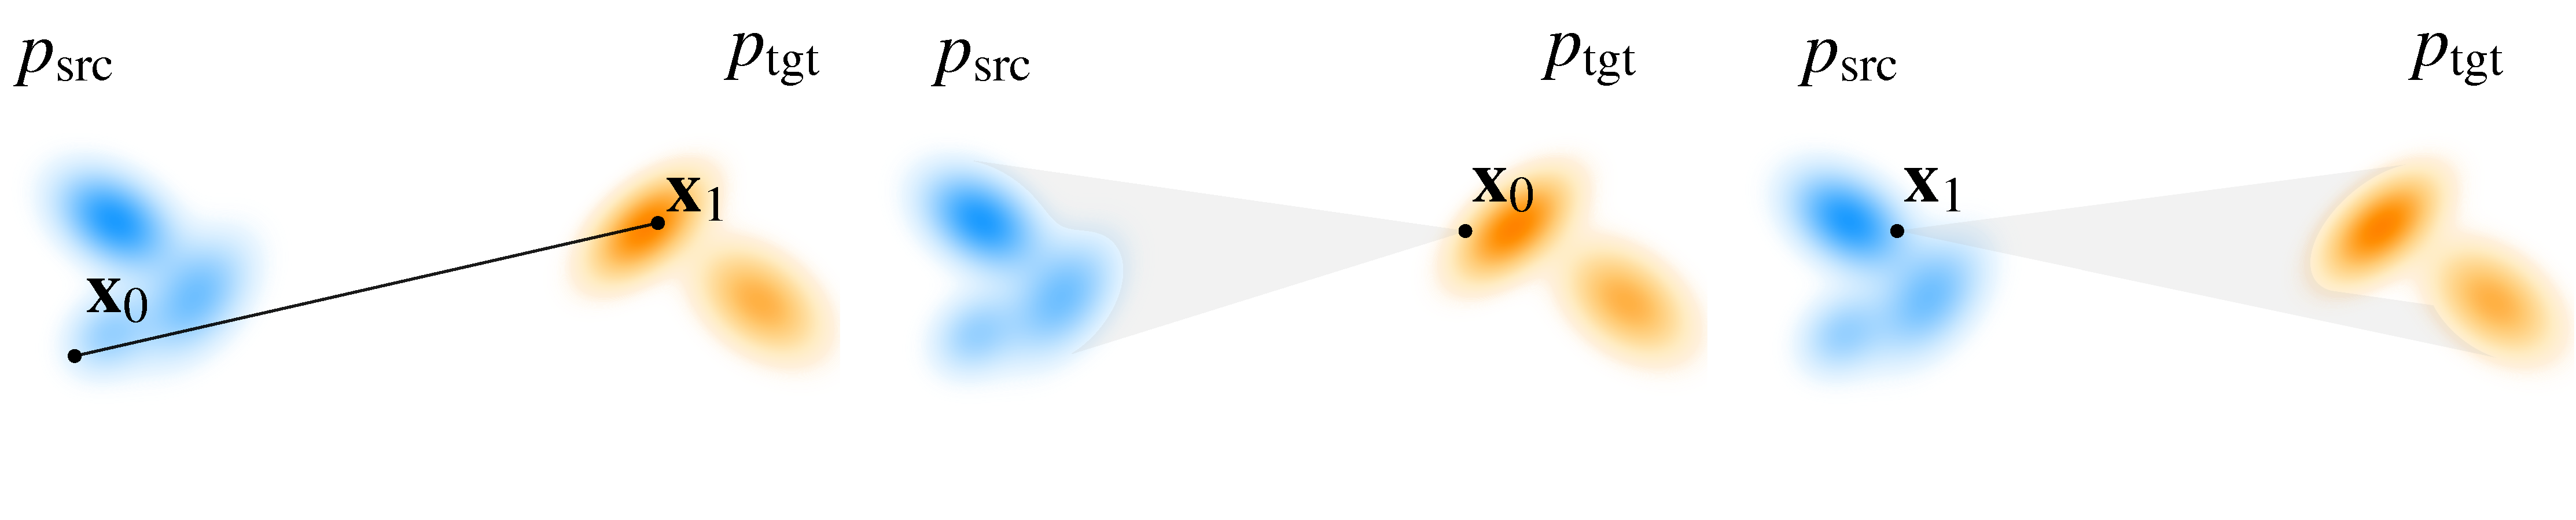
\includegraphics[width=\linewidth]{Images/PartB/triptych_gray_cones_final.pdf}
    \caption{\textbfs{Illustrations of two common types of conditioning probability paths}. It includes:
(i) \emph{two-sided}, conditioned on $\rvx_0 \sim p_{\text{tgt}}$ and $\rvx_1 \sim p_{\text{src}}$ with general endpoint distributions; 
(ii) \emph{one-sided}, conditioned at either $\rvx_0 \sim p_{\text{tgt}}$ or $\rvx_1 \sim p_{\text{src}}$.
\figcredit{Created by the authors.}}
    \label{fig:conditional-path}
\end{figure}

We aim to construct a conditional density path $p_t(\cdot|\rvz)$ first and then derive its corresponding conditional velocity field $\rvv_t(\cdot|\rvz)$ (via Proposition~\ref{closed-form-vf}), under conditioning with respect to $\pi(\rvz)$. 
Depending on how $\rvz$ is chosen, there are two natural scenarios: 
(i) two-sided conditioning with $\rvz=(\rvx_0,\rvx_1)$, or 
(ii) one-sided conditioning with $\rvz=\rvx_0$ or $\rvx_1$. 
In either case, the construction must match the boundary distributions:
\begin{align*}
   p_{\mathrm{src}}(\rvx_0) = \int p_0(\rvx_0|\rvz) \pi(\rvz)\diff\rvz, \quad
   p_{\mathrm{tgt}}(\rvx_1) = \int p_1(\rvx_1|\rvz) \pi(\rvz) \diff\rvz.
\end{align*}
Since verifying these constraints is straightforward once a concrete construction is specified, we do not emphasize the verification step here.


 
\paragraph{I. Two-Sided $\rvz = (\rvx_0, \rvx_1)$ — ``Beam-Like'' Path.}
    \subparagraph{Choice of $\pi(\rvz)$.} Consider general distributions $p_{\mathrm{src}}$ and $p_{\mathrm{tgt}}$ over $\mathbb{R}^D$. Let $\rvz = (\rvx_0, \rvx_1)$ with $\rvx_0 \sim p_{\mathrm{src}}$ and $\rvx_1 \sim p_{\mathrm{tgt}}$ independently, i.e.,
    \[
    \pi(\rvz) = p_{\mathrm{src}}(\rvx_0)  p_{\mathrm{tgt}}(\rvx_1).
    \]
    \subparagraph{Choice of Conditional Path $p_t(\cdot|\rvz)$.} Define the conditional path by linear interpolation with a fixed and small variance $\sigma > 0$\footnote{
One may instead add a fixed conditional variance $\sigma^2\rmI$.
The conditional velocity remains $a_t'\rvx_0+b_t'\rvx_1$ because the
variance is constant in time, but the endpoint marginals then become Gaussian
smoothings of $p_{\mathrm{src}}$ and $p_{\mathrm{tgt}}$, approaching the
desired endpoints as $\sigma\to0$.
}:
    \[
    p_t(\rvx_t | \rvz = (\rvx_0, \rvx_1)) = \mathcal{N}(\rvx_t; a_t\rvx_0 + b_t\rvx_1,  \sigma^2 \rmI),
    \]
    where $a_t$ and $b_t$ are time-dependent functions satisfying  $a_0 = 1,  b_0 = 0$ and $a_1 = 0,  b_1 = 1$. A choice suggested by \citep{lipman2022flow,liu2022rectified} is $a_t = 1-t$, $b_t = t$.  In the deterministic case $\sigma = 0$, we obtain  
\[
p_t(\rvx_t |\rvz) = \delta \big(\rvx_t - [a_t\rvx_0 + b_t\rvx_1]\big),
\]
which describes a deterministic interpolating path from $\rvx_0$ to $\rvx_1$.
    \subparagraph{Derived Conditional Velocity  $\rvv_t(\cdot|\rvz)$.} By Proposition~\ref{closed-form-vf}, the conditional velocity is
    \[
    \rvv_t(\rvx | \rvz) = a'_t\rvx_0 + b'_t\rvx_1.
    \]
    \subparagraph{CFM Loss.} When $\sigma=0$ so that $\rvx_t = a_t\rvx_0 + b_t\rvx_1$, the CFM loss reduces to
    \[
    \mathcal{L}_{\mathrm{CFM}} = \mathbb{E}_{t, \rvx_0\sim p_{\text{src}}, \rvx_1\sim p_{\text{tgt}}} \left\| \rvv_{\bm{\phi}}(\rvx_t, t) - \left(a'_t\rvx_0 + b'_t\rvx_1\right) \right\|^2.
    \]
From \Cref{eq:marginal-oracle-velocity,eq:minimum_velocity}, the optimal velocity field is
\[
\rvv^*(\rvx_t, t) = \mathbb{E} \left[ \rvx_t'|\rvx_t \right] = \mathbb{E} \left[ a'_t\rvx_0 + b'_t\rvx_1|\rvx_t \right].
\]
Here, the expectation is taken over $p(\mathbf{x}_0, \mathbf{x}_1|\mathbf{x}_t)$, the conditional distribution over source-target pairs $(\mathbf{x}_0, \mathbf{x}_1)$ that could have produced the observed interpolation $\mathbf{x}_t = a_t\mathbf{x}_0 + b_t\mathbf{x}_1$ at time $t$.



\paragraph{II. One-Sided $\rvz = \rvx_0$ or $\rvx_1$ — ``Spotlight-Like'' Path.}
We illustrate the conditional probability–path–first construction in the one-sided setting, considering the standard generative setup with $p_{\mathrm{src}}=\mathcal N(\bm 0,\rmI)$ and $p_{\mathrm{tgt}}=p_{\mathrm{data}}$.
Crucially, this Gaussian source is not an additional assumption but a direct consequence of the conditional path defined below.
A more general treatment of arbitrary endpoints will be given in \Cref{subsec:prob-path-flow}.

\subparagraph{Choice of $\pi(\rvz)$.}
We take $\rvz=\rvx_1$ with $\pi(\rvz)=p_{\mathrm{data}}(\rvx_1)$ (the case $\rvz=\rvx_0\sim p_{\mathrm{prior}}$ follows analogously).

\subparagraph{Choice of Conditional Path $p_t(\cdot|\rvz)$.}
For fixed $\rvx_1\sim p_{\mathrm{data}}$, define
\[
p_t(\rvx_t|\rvz=\rvx_1)=\mathcal N \big(\rvx_t; b_t \rvx_1, a_t^2 \rmI\big),
\]
with $ a_0=1, b_0=0, a_1=0, b_1=1$ (usually interpreted as the limit).
At the boundaries,
\[
p_0(\cdot|\rvz=\rvx_1)=\mathcal N(\cdot; \bm 0,\rmI),\qquad
p_1(\cdot|\rvz=\rvx_1)=\delta(\cdot - \rvx_1).
\]
Marginalizing over $\rvx_1$ yields $\{p_t\}_{t\in[0,1]}$ with
$p_0=\mathcal N(\bm 0,\rmI)$ (independent of $p_{\mathrm{data}}$) and $p_1=p_{\mathrm{data}}$.

\subparagraph{Derived Conditional Velocity  $\rvv_t(\cdot|\rvz)$.}
For $t\in(0,1)$ with $a_t>0$, applying Proposition~\ref{closed-form-vf} to the conditional Gaussian path gives
\[
\mathbf v_t(\rvx|\rvx_1)
= b_t' \rvx_1 + \frac{a_t'}{a_t} \big(\rvx - b_t \rvx_1\big).
\]

\subparagraph{One-Sided CFM Objective.}
With $t\sim\mathcal U(0,1)$ (or any fixed sampling distribution) and $\rvx_1\sim p_{\mathrm{data}}$, the CFM loss becomes
\begin{align}\label{eq:one-sided-cfm}
    \mathcal L_{\mathrm{CFM}}
=\E_{t,\rvx_1} \E_{\rvx_t\sim p_t(\cdot|\rvx_1)}
\Big\|\mathbf v_\phi(\rvx_t,t)-
\Big[b_t'\rvx_1+\tfrac{a_t'}{a_t}\big(\rvx_t-b_t\rvx_1\big)\Big]\Big\|_2^2.
\end{align}
By MSE optimality, the unique minimizer is the marginal velocity field
\[
\mathbf v^*(\rvx,t)
= \E \left[\mathbf v_t(\rvx|\rvx_1) |dle|  \rvx_t=\rvx\right]
= \E \left[a_t'\rvx_0+b_t'\rvx_1 |dle|  \rvx_t=\rvx\right].
\]

\subparagraph{Equivalence to Two-Sided Target.}
For paired samples $(\rvx_0,\rvx_1)$ with $\rvx_t=a_t\rvx_0+b_t\rvx_1$,
\[
\mathbf v_t(\rvx_t|\rvx_1)
= b_t'\rvx_1 + \tfrac{a_t'}{a_t}\big(\rvx_t-b_t\rvx_1\big)
= a_t'\rvx_0 + b_t'\rvx_1.
\]
Thus the one-sided loss regresses to the \emph{conditional expectation} of the two-sided target given $\rvx_t$:
\[
\mathbf v^*(\rvx,t)=\E \big[a_t'\rvx_0 + b_t'\rvx_1 | \rvx_t=\rvx\big],
\]
so the one-sided and two-sided CFM objectives share the same minimizer.


\paragraph{Gaussian FM = Diffusion Model.}
We use the FM convention where $t=0$ denotes the source/prior and $t=1$ denotes the target/data:
\[
p_{\mathrm{src}}=p_{\mathrm{prior}},\qquad p_{\mathrm{tgt}}=p_{\mathrm{data}}.
\]
By contrast, diffusion models typically index time from data to noise (i.e., $t=0$ is data and $t=1$ is prior). 
Here, we adopt the FM convention indexing in the main discussion. For comparison, however, the VE and VP entries in \Cref{tb:interpolant_instances} are summarized in their usual diffusion-time indexing, where $t=0$ corresponds to data and $t=1$ to prior/noise.
If further $p_{\mathrm{src}}=\mathcal N(\bm 0,\rmI)$, then for fixed condition $\rvx_1\sim p_{\mathrm{data}}$, 
the conditional path $p_t(\cdot |\rvx_1)$ is naturally chosen to be Gaussian, 
while the target distribution $p_{\mathrm{tgt}}$ itself need not be Gaussian. We refer to this Gaussian conditional-path setting as \emph{Gaussian FM}.
Diffusion probability paths form an important subclass of such Gaussian
paths. A generic Gaussian schedule, however, need not correspond to a valid
forward diffusion SDE; the schedule must additionally satisfy the SDE
compatibility condition in Lemma~\ref{forward-sde}.



Choosing $a_t = 1-t$ and $b_t = t$ (equivalently, $\alpha_t = t$ and $\sigma_t = 1-t$ under the relabeling $a_t:=\sigma_t$, $b_t:=\alpha_t$ in diffusion model) recovers the familiar FM/RF schedule~\citep{lipman2022flow,liu2022rectified}.


\begin{table}[th]
\caption{Summary of different interpolants written as
$\rvx_t=a_t\rvx_0+b_t\rvx_1$, where
$\rvx_0\sim p_{\mathrm{src}}=p_{\mathrm{prior}}$ and
$\rvx_1\sim p_{\mathrm{tgt}}=p_{\mathrm{data}}$.
The FM/RF and trigonometric columns use the FM convention
($t=0$ source, $t=1$ target), whereas the VE/VP columns retain the usual
diffusion-time convention ($t=0$ data, $t=1$ prior/noise), with
$a_t:=\sigma_t$ and $b_t:=\alpha_t$.
For VE at a finite terminal noise level, the exact terminal marginal is
$p_{\mathrm{data}}*\mathcal{N}(\bm{0},a_1^2\rmI)$; the Gaussian prior shown
in the table is the usual approximation when the terminal noise dominates
the scale of the data.}
  \small
  \centering
  \resizebox{\textwidth}{!}{
  \begin{tabular}{lcccc}
     \toprule
         & \textbfs{VE} & \textbfs{VP} & \textbfs{FM/RF} & \textbfs{Trig.}~\citep{albergo2023stochastic} \\
    \midrule
     $a_t$ (prior coeff.) 
       & $a_t$ 
       & $\sqrt{1-b_t^2}$ 
       & $1-t$ 
       & $\cos \bigl(\tfrac{\pi}{2}t\bigr)$ \\
     $b_t$ (data coeff.) 
       & $1$ 
       & $b_t$ 
       & $t$ 
       & $\sin \bigl(\tfrac{\pi}{2}t\bigr)$ \\
    \midrule
     $a_0$ & $0$ & $0$ & $1$ & $1$ \\
     $b_0$ & $1$ & $1$ & $0$ & $0$ \\
     $a_1$ & $a_1$ & $1$ & $0$ & $0$ \\
     $b_1$ & $1$ & $0$ & $1$ & $1$ \\
    \midrule
     $p_{\text{prior}}$ 
       & $p_{\mathrm{data}} * \mathcal{N}(\bm{0},a_1^2\rmI)
   \approx \mathcal{N}(\bm{0},a_1^2\rmI)$ 
       & $\mathcal{N}(\bm{0},\rmI)$ 
       & $\mathcal{N}(\bm{0},\rmI)$ 
       & $\mathcal{N}(\bm{0},\rmI)$ \\
     \bottomrule
  \end{tabular}}
  \label{tb:interpolant_instances}
\end{table}



In the Gaussian FM setting, both the beam-like and spotlight-like conditional paths lead to training objectives that are  similar to the standard diffusion losses. As we will elaborate in \Cref{ch:all-equivalent}, Gaussian FM can in fact be equivalently interpreted as a diffusion model trained to predict the \emph{velocity}, under the linear schedule $a_t = 1-t$ and $b_t = t$. This perspective highlights that flow matching and diffusion are not fundamentally different, but rather two equivalent formulations that can be transformed into one another. The Gaussian FM objective is particularly appealing in practice: its loss function ($\E_{t,\rvx_t} \left[\norm{\rvv_\bphi(\rvx_t, t) - (\rvx_1 - \rvx_0)}_2^2\right]$) is simple, and it has been shown to achieve competitive performance at scale~\citep{esser2024scaling}. 




\subsection{Conditional Flow-First Construction of $\rvv_t(\cdot|\rvz)$ and $p_t(\cdot|\rvz)$}\label{subsec:prob-path-flow}

We treat the general case where the endpoints $p_{\mathrm{src}}$ (at $t=0$) and $p_{\mathrm{tgt}}$ (at $t=1$) are arbitrary. 
Our goal is to design, directly in trajectory space, a conditional flow that transports samples from $p_{\mathrm{src}}$ to $p_{\mathrm{tgt}}$ and yields a closed-form $\rvv_t(\rvx_t|\rvz)$ usable as a regression target.

\paragraph{Motivation.}
Instead of first designing conditional density path, we may directly specify a conditional flow map $\bPsi_{0\to t}(\cdot;\rvz)$ that moves samples along trajectories. This has two practical advantages: (i) it immediately yields a regression target for training via a time derivative along trajectories; (ii) on geometry-structured spaces (Riemannian manifolds, Lie groups, or constrained submanifolds), it is often natural to construct the conditional flow map 
$\bPsi_{0\to t}$ directly from the geometry (e.g., geodesics, exponential maps, or premetrics)~\citep{lipman2024flow} which yields analytic, simulation-free target velocities for training.


\paragraph{Conditional Affine Flow (Link to Proposition~\ref{closed-form-vf}).}
We fix a conditioning variable $\rvz\sim\pi$ (e.g., $\rvz=\rvx_1\sim p_{\mathrm{tgt}}$ in one-sided “spotlight’’ training) and push forward $\rvx_0\sim p_{\mathrm{src}}$ through the time-varying \emph{conditional affine flow} 
\[
\bPsi_{0\to t}(\rvx_0;\rvz) := \bm\mu_t(\rvz) + \rmA_t(\rvz) \rvx_0,\qquad t\in[0,1],
\]
where $\bm\mu_t(\rvz)\in\R^D$ and $\rmA_t(\rvz)\in\R^{D\times D}$ is invertible for $t\in(0,1)$. The boundary 
$\rmA_0(\rvz)=\rmI,\ \bm\mu_0(\rvz)=\mathbf 0$ recovers $p_{\mathrm{src}}$ at $t=0$. It is standard to interpret boundary when $t\to1$ as a limit (the terminal map may concentrate mass on a lower-dimensional set or a point)\footnote{Allowing $\rmA_1(\rvz)$ to be singular (e.g., $\mathbf 0$) is compatible with invertibility on $(0,1)$ and causes the path to contract onto the prescribed endpoint at $t=1$.}. 


\subparagraph{Induced Conditional Path $p_t(\cdot|\rvz)$.}
The construction defines
\[
p_t(\cdot|\rvz) = \bigl(\bPsi_{0\to t}( \cdot ;\rvz)\bigr)_{\#} p_{\mathrm{src}},
\qquad
p_t(\cdot)  =  \int p_t(\cdot|\rvz)\pi(\rvz)\diff\rvz.
\]
What ultimately matters in $\mathcal{L}_{\mathrm{CFM}}$ is how to sample from it:  
first draw $\rvz \sim \pi$, then draw $\rvx_0 \sim p_{\mathrm{src}}$, and finally set
\[
\rvx_t = \bm\mu_t(\rvz) + \rmA_t(\rvz)\rvx_0.
\]


We remark that when $\bPsi_{0\to t}$ is affine in $\rvx_0$, then $p_t( \cdot | \rvz)$ is Gaussian 
if and only if $p_{\mathrm{src}}$ is Gaussian. 
In particular, for arbitrary (non-Gaussian) $p_{\mathrm{src}}$, an affine flow yields a
generally non-Gaussian $p_t(\cdot|\rvz)$.


\subparagraph{Derived Conditional Velocity $\rvv_t(\cdot|\rvz)$.} The conditional velocity $\rvv_t(\cdot|\rvz)$ is obtained by $t$-differentiating the conditional flow map $\bPsi_{0\to t}$. Following the derivation in Proposition~\ref{closed-form-vf}, consider the \emph{conditional} ODE defined by the flow map $\bPsi_{0\to t}(\rvy;\rvz)$ with initial condition $\rvy$, where the goal is to identify the corresponding conditional velocity field $\rvv_t(\cdot|\rvz)$:
\[
\frac{\diff}{\diff t} \bPsi_{0\to t}(\rvy;\rvz)
= \rvv_t \Big(\underbrace{\bPsi_{0\to t}(\rvy;\rvz)}_{\rvx} \Big| \rvz\Big).
\]
Since $\bPsi_{0\to t}(\cdot;\rvz)$ is invertible for $t\in(0,1)$, we may
express the initial point $\rvy$ corresponding to the current state
$\rvx=\bPsi_{0\to t}(\rvy;\rvz)$ as
\[
\rvy
=
\bPsi_{0\to t}^{-1}(\rvx;\rvz)
=
\bPsi_{t\to0}(\rvx;\rvz).
\]
The corresponding Eulerian velocity field is therefore
\[
\rvv_t(\rvx|\rvz)
:=
\left.
\frac{\partial}{\partial t}
\bPsi_{0\to t}(\rvy;\rvz)
\right|_{\rvy=\bPsi_{0\to t}^{-1}(\rvx;\rvz)}.
\]
That is, we first differentiate the forward flow map with respect to $t$
while holding its initial point $\rvy$ fixed, and then substitute the initial
point whose trajectory reaches $\rvx$ at time $t$.


Since $\rvx_t=\bm\mu_t(\rvz)+\rmA_t(\rvz)\rvx_0$ and $\rmA_t(\rvz)$ is invertible on $(0,1)$, we have $\rvx_0=\rmA_t(\rvz)^{-1}\bigl(\rvx-\bm\mu_t(\rvz)\bigr)$, giving
\[
\rvv_t(\rvx|\rvz)
 = 
\bm\mu_t'(\rvz) + \rmA_t'(\rvz) \rmA_t(\rvz)^{-1} \bigl(\rvx-\bm\mu_t(\rvz)\bigr).
\]


\subparagraph{One-Sided Conditioning ($\rvz=\rvx_1$).}
Choosing $\bm\mu_t(\rvz)=b_t \rvz$ and $\rmA_t(\rvz)=a_t \rmI$ with $a_0=1,a_1=0$ and $b_0=0,b_1=1$ (with $a_t>0$ for $t\in(0,1)$) yields
\[
\rvx_t = a_t \rvx_0 + b_t \rvx_1,
\qquad
\rvv_t(\rvx|\rvx_1) = b_t' \rvx_1 + \frac{a_t'}{a_t} \bigl(\rvx-b_t\rvx_1\bigr).
\]
On paired samples $(\rvx_0,\rvx_1)$ (with $\rvx_t=a_t\rvx_0+b_t\rvx_1$), this simplifies to the usual CFM target:
\[
\rvv_t(\rvx_t|\rvx_1)=a_t' \rvx_0 + b_t' \rvx_1.
\]

\subparagraph{Two-Sided Conditioning ($\rvz=(\rvx_0,\rvx_1)$).}
The same template with $\bm\mu_t(\rvx_0,\rvx_1)=b_t \rvx_1$ and $\rmA_t(\rvx_0,\rvx_1)=a_t \rmI$ makes the conditional path \emph{deterministic}:
\[
\rvx_t=a_t \rvx_0+b_t \rvx_1,
\qquad
p_t(\cdot|\rvx_0,\rvx_1)=\delta\left(\cdot - (a_t\rvx_0+b_t\rvx_1)\right),
\]
and the conditional velocity is
\[
\rvv_t(\rvx_t|\rvx_0,\rvx_1)=a_t' \rvx_0+b_t' \rvx_1,
\]
i.e., the standard two-sided CFM target. 

\subparagraph{Unconditional Gaussian Path as a Special Case.}
If $\bm{\mu}_t$ is independent of $\rvz$ (denoted $\bm{\mu}(t)$) and 
$\rmA_t = \tfrac{\sigma(t)}{\sigma(0)} \rmI$, then
\[
\bPsi_{0\to t}(\rvx_0)=\bm\mu(t)+\sigma(t) \frac{\rvx_0-\bm\mu(0)}{\sigma(0)},
\quad
\rvv_t(\rvx)=\bm\mu'(t)+\frac{\sigma'(t)}{\sigma(t)}\bigl(\rvx-\bm\mu(t)\bigr),
\]
which recovers the Gaussian density path and the closed-form velocity in Proposition~\ref{closed-form-vf}.





\subsection{Probability-Path-First vs. Flow-First Construction}

The two constructions correspond to complementary Eulerian and Lagrangian
descriptions of transport. The \emph{probability-path-first} (Eulerian)
view begins by specifying a conditional density path
$p_t(\cdot|\rvz)$ and then selects a compatible velocity field through the
continuity equation. Because a density path alone generally does not
determine the velocity uniquely, additional transport structure may be
needed to select one.

The \emph{flow-first} (Lagrangian) view instead specifies a conditional
flow map $\bPsi_{0\to t}(\cdot|\rvz)$, which directly describes particle
trajectories. The corresponding density path follows by pushforward, and
when the map is invertible its Eulerian velocity is uniquely recovered as
\[
\rvv_t
=
\partial_t\bPsi_{0\to t}
\circ
\bPsi_{0\to t}^{-1}.
\]
Both constructions therefore describe the same kinds of transport objects
from different starting points, but a prescribed density path need not
select the same velocity as a separately prescribed flow map.

The following table summarizes these contrasts. The takeaway: path-first is natural when conditional paths admit closed-form velocities; flow-first is natural when you have strong structural priors on trajectories.


\begin{table}[th!]
\caption{Comparison of conditional probability-path-first and conditional flow-first constructions.}
\label{tb:conditional-path-vs-flow}
\centering
\begingroup
\scriptsize
\setlength{\tabcolsep}{4pt}
\renewcommand{\arraystretch}{1.05}
\begin{tabular}{p{0.13\linewidth} p{0.41\linewidth} p{0.41\linewidth}}
\toprule
\textbfs{Axis}
&
\textbfs{Conditional Probability-Path-First}
&
\textbfs{Conditional Flow-First}
\\
\midrule

\textbfs{Given}
&
Conditional density path $p_t(\cdot|\rvz)$.
&
Conditional flow map $\bPsi_{0\to t}(\cdot|\rvz)$
(trajectories, for each fixed $\rvz$).
\\

\graymidrule

\textbfs{Get Velocity}
&
For each $\rvz$, find $\rvv_t(\cdot|\rvz)$ s.t.\
$$
\partial_t p_t(\cdot|\rvz)
+
\nabla \cdot
\left(
p_t(\cdot|\rvz)\rvv_t(\cdot|\rvz)
\right)
=
0;
$$
Non-unique: if
$\nabla\!\cdot~\left(p_t \mathbf w_t\right)=0$
then $\rvv_t+\mathbf w_t$ yields the same $p_t$.
&
Along paths (for each $\rvz$):
$$
\rvv_t
\left(
\bPsi_{0\to t}(\cdot|\rvz)
\mid
\rvz
\right)
=
\tfrac{\diff}{\diff t}
\bPsi_{0\to t}(\cdot|\rvz).
$$
When $\bPsi_{0\to t}$ is invertible, one can solve
$$
\rvv_t(\rvx|\rvz)
=
\left.
\partial_t
\bPsi_{0\to t}(\rvy|\rvz)
\right|_{\rvy=\bPsi_{0\to t}^{-1}(\rvx|\rvz)}.
$$
\\

\graymidrule

\textbfs{Closed Form \newline of $\rvv_t(\cdot|\rvz)$}
&
Convenient when $p_t(\cdot|\rvz)$ is Gaussian / exponential-family;
otherwise obtaining $\rvv_t(\cdot|\rvz)$ is nontrivial.
&
Convenient when $\bPsi_{0\to t}(\cdot|\rvz)$ has structure
(affine/low-rank); avoids density evaluation.
\\

\graymidrule

\textbfs{Uniqueness \newline of $\rvv_t(\cdot|\rvz)$}
&
For each $\rvz$, $\rvv_t(\cdot|\rvz)$ is underdetermined unless a
selection rule (e.g., potential flow / min.\ kinetic energy) is imposed.
&
Given $\bPsi_{0\to t}(\cdot|\rvz)$, both
$p_t(\cdot|\rvz)=(\bPsi_{0\to t}(\cdot|\rvz))_\#p_0$
and the particle trajectories are determined. If the flow map is invertible,
the corresponding Eulerian velocity field is uniquely determined; otherwise,
a unique global Eulerian field need not exist.
\\

\graymidrule

\textbfs{Realizability}
&
Must verify the constructed $\rvv_t(\cdot|\rvz)$ solving the continuity
equation on the intended support.
&
Holds by construction:
$$
p_t(\cdot|\rvz)
=
\left(
\bPsi_{0\to t}(\cdot|\rvz)
\right)_\#
p_0(\cdot|\rvz).
$$
\\

\graymidrule

\textbfs{Match \newline $(p_{\mathrm{src}},p_{\mathrm{tgt}})$}
&
Mix conditionals:
\newline
\hspace{3cm}
$p_{\mathrm{src}}
=
\int p_0(\cdot|\rvz)\pi(\rvz)\diff\rvz,$
\newline
$p_{\mathrm{tgt}}
=
\int p_1(\cdot|\rvz)\pi(\rvz)\diff\rvz.$
\newline
Under Gaussian--affine conditional paths with $\rvz$-independent coefficients,
$p_{\mathrm{src}}$ can be forced to be Gaussian.
For a general fixed endpoint $p_{\mathrm{src}}$ (possibly non-Gaussian),
the choice of $p_t(\cdot|\rvz)$ does not generally pin $p_{\mathrm{src}}$.
&
Set $\bPsi_{0\to 0}=\mathrm{Id}$ and choose boundary condition to hit any
$p_{\mathrm{tgt}}$.
\\

\graymidrule

\textbfs{Preferred \newline Scenarios}
&
Diffusion-style constructions; analytic targets via conditional Gaussians
$p_t(\cdot|\rvz)$.
&
Strong structural priors via maps $\bPsi_{0\to t}(\cdot|\rvz)$;
easy boundary control; accommodates singular/low-dimensional endpoints;
natural for map-based regularization/transport costs.
\\

\bottomrule
\end{tabular}
\endgroup
\end{table}





%%%%%%%%%%%%%%%%%
\subsection{Conditional Straightness Does Not Imply Marginal-Flow
Straightness}

The canonical affine interpolation
\[
\rvx_t
=
(1-t)\rvx_0+t\rvx_1
\]
has an appealing geometric property: conditioned on a particular
endpoint pair $(\rvx_0,\rvx_1)$, the interpolation is a straight line
with constant velocity $\rvx_1-\rvx_0$.
This conditional notion of straightness is used extensively in Flow
Matching and Rectified Flow.

It is important, however, to distinguish the straightness of these
\emph{conditional interpolation paths} from the straightness of the
\emph{marginal ODE trajectories} used at generation time.
Under a coupling $\pi(\rvx_0,\rvx_1)$, the population-optimal marginal
velocity is
\[
\rvv^\star(\rvx,t)
=
\mathbb{E}
\left[
\rvx_1-\rvx_0
\,\middle|\,
\rvx_t=\rvx
\right].
\]
The posterior over endpoint pairs generally changes with $(\rvx,t)$.
Consequently, the velocity encountered along a marginal ODE trajectory
need not remain constant, even though every conditional interpolation
used for training is a straight line.

Thus, choosing the canonical affine schedule alone does not imply that
the learned marginal ODE is exactly straight or that one Euler step is
exact. Rectified Flow addresses precisely this distinction: its
rectification or \texttt{Reflow} procedure changes the endpoint coupling
so that the induced causal flow can become progressively closer to a
straight flow~\citep{liu2022flow}.

The following example makes the distinction explicit.

\exm{A Simple 1D Counterexample}{
Consider the one-dimensional setting with
\[
x_0 \sim \mathcal{N}(0, \sigma_0^2),
\qquad
x_1 \sim \mathcal{N}(0, \sigma_1^2),
\]
independent coupling, and the canonical affine interpolation
$x_t = (1-t)x_0 + tx_1$.
Each conditional path $(1-t)x_0 + tx_1$ is a straight line in
time. We now compute the induced marginal velocity field.

Since $(x_1 - x_0,\, x_t)$ is jointly Gaussian, the
conditional expectation is linear in $x$, so
\[
v^*(x,t)
= \E[x_1 - x_0| x_t = x]
= \frac{\operatorname{Cov}(x_1 - x_0,\, x_t)}
       {\operatorname{Var}(x_t)}\, x.
\]
A direct calculation gives
\[
\operatorname{Var}(x_t)
= (1-t)^2\sigma_0^2 + t^2\sigma_1^2
=: V(t),
\]
and
\[
\operatorname{Cov}(x_1 - x_0,\, x_t)
= t\sigma_1^2 - (1-t)\sigma_0^2
= \tfrac{1}{2} V'(t).
\]
Hence
\[
v^*(x,t) = \frac{V'(t)}{2V(t)}\, x.
\]

The marginal ODE
\[
\frac{\diff z_t}{\diff t} = v^*(z_t, t)
\]
therefore has the exact solution
\[
z_t
= z_0 \sqrt{\frac{V(t)}{V(0)}}
= z_0 \sqrt{(1-t)^2 + \frac{\sigma_1^2}{\sigma_0^2}\, t^2}.
\]

Now, a straight-line interpolation in time would require $z_t$ to be
affine in $t$, namely $z_t = (1-t)z_0 + t\,z_1$ for some endpoint
$z_1$. But
\[
\sqrt{(1-t)^2 + \frac{\sigma_1^2}{\sigma_0^2}\, t^2}
\]
is not affine in $t$ for any positive $\sigma_0, \sigma_1$. Thus the ODE
trajectory is generally not a straight-line interpolation in time. We illustrate this phenomenon in \Cref{fig:straightness-counterexample}
with the example $\sigma_0=2$ and $\sigma_1=3$.

For example, when $\sigma_0 = \sigma_1$, we have $z_1 = z_0$, so a
straight-line interpolation would simply be the constant path
$z_t = z_0$. In contrast, the actual ODE trajectory satisfies
\[
z_{1/2} = \frac{z_0}{\sqrt{2}} \neq z_0.
\]
Therefore, even though every conditional interpolation path is straight,
the induced marginal ODE trajectory need not be.
}
%%%%%%%%%%%%%

\begin{figure}[th]
        \label{fig:straightness-counterexample}
    \centering
    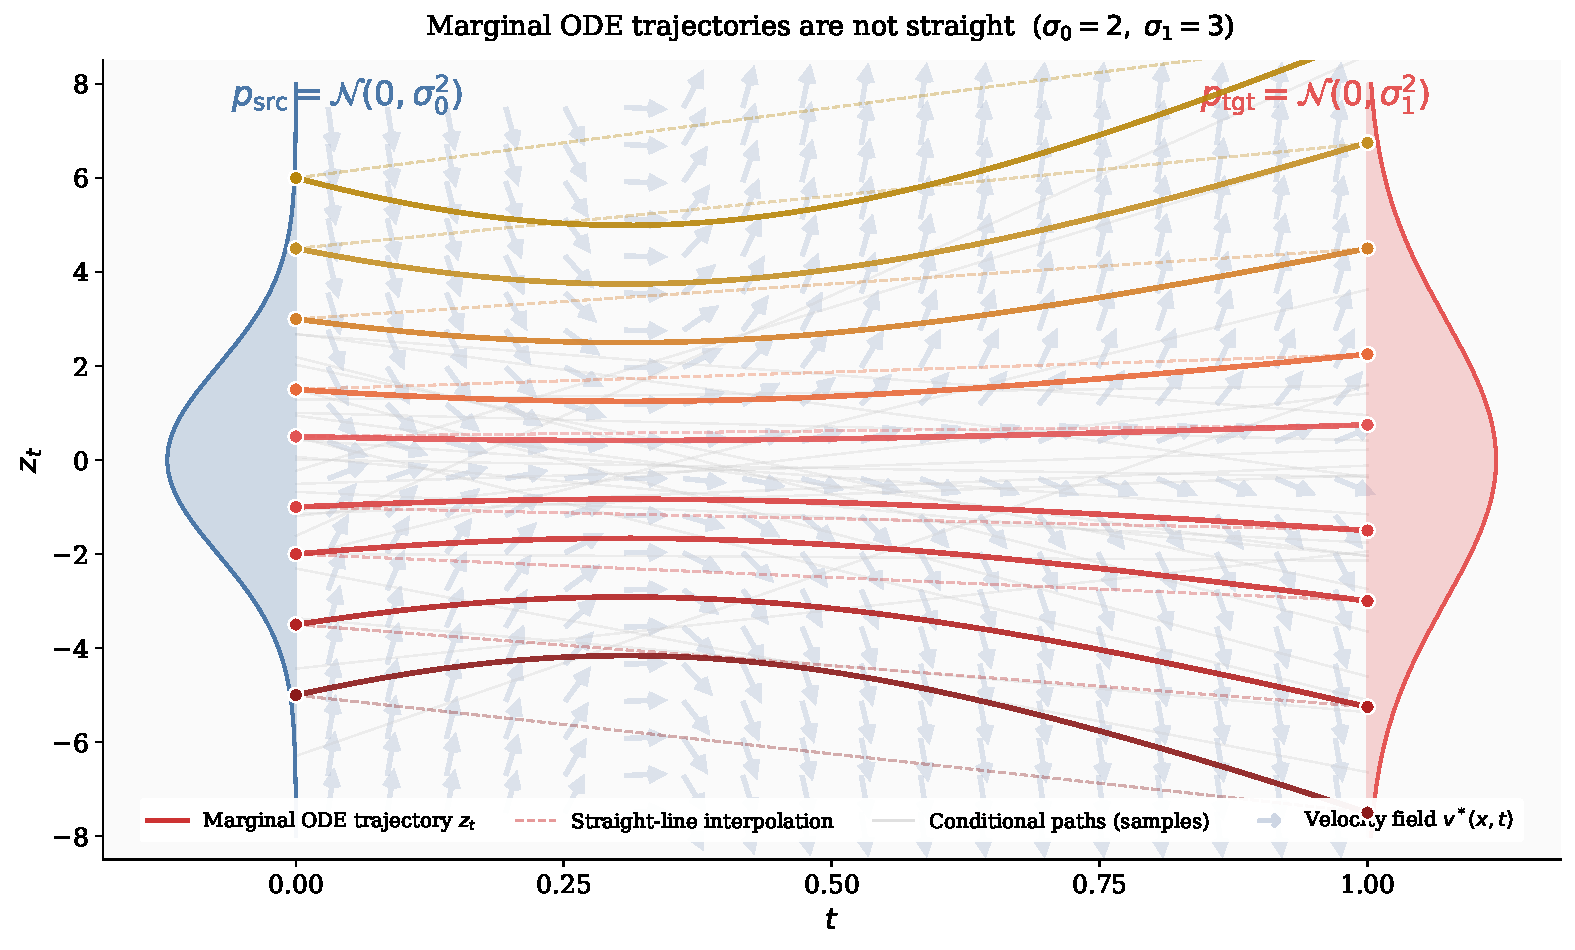
\includegraphics[width=\linewidth]{Images/PartB/straightness_counterexample.pdf}
    \caption{\textbfs{Marginal ODE trajectories are not straight under the canonical affine interpolation.}
    We take $x_0 \sim \mathcal{N}(0, \sigma_0^2)$ and $x_1 \sim \mathcal{N}(0, \sigma_1^2)$ with $\sigma_0=2$, $\sigma_1=3$, and independent coupling.
    Gray lines show sampled conditional paths $(1-t)x_0 + tx_1$, which are straight by construction.
    Solid curves show the exact marginal ODE trajectories $z_t = z_0\sqrt{(1-t)^2 + (\sigma_1/\sigma_0)^2 t^2}$, and dashed lines show the corresponding straight-line interpolations from $z_0$ to $z_1$.
    The visible gap between solid and dashed curves confirms that the marginal ODE trajectories are not affine in $t$, even though every conditional path is a straight line.
    The marginal densities $p_{\mathrm{src}}$ and $p_{\mathrm{tgt}}$ are shown on the left and right margins, respectively.
    \figcredit{Created by the authors with AI-assisted coding.}}
\end{figure}
     





%%%%%%%%%%%%%%%%%%%%%%%%%%%%%%%%%%%%%%%%%%%%%%%%%%%%%%%%%%%%%%%%%%%%%%%%
\clearpage
\newpage
%%%%%%%%%%%%%%%%%%%%%%%%%%%%%%%%%%%%%%%%%%%%%%%%%%%%%%%%%%%%%%%%%%%%%%%%

\section{\texorpdfstring{(Optional) Properties of the Canonical Affine Flow}{(Optional) Properties of the Canonical Affine Flow}}\label{sec:optimal-canonical}

Given two endpoint distributions $p_0=p_{\mathrm{src}}$ and $p_1=p_{\mathrm{tgt}}$, 
a natural and widely used choice for defining the conditional path in flow matching (FM)~\citep{lipman2022flow} 
and rectified flow (RF)~\citep{liu2022flow} is the linear interpolation
\[
a_t = 1 - t, \qquad b_t = t,
\]
which yields the interpolant
\[
\mathbf{x}_t = (1 - t)\mathbf{x}_0 + t \mathbf{x}_1, 
\qquad \mathbf{x}_0 \sim p_{\mathrm{src}},\ \mathbf{x}_1 \sim p_{\mathrm{tgt}}.
\]
Under this choice, the training objective simplifies to
\[
\mathbb{E}_{t \sim \mathcal{U}[0,1]}   
\mathbb{E}_{\mathbf{x}_0, \mathbf{x}_1} 
\left[ \bigl\|\mathbf{v}_{\bm{\phi}}(\mathbf{x}_t, t) - (\mathbf{x}_1 - \mathbf{x}_0)\bigr\|_2^2 \right].
\]

This linear flow enjoys several appealing properties. 
In particular, it admits an iterative refinement scheme, known as \emph{\texttt{Reflow}}, 
which progressively straightens the path between distributions while preserving the marginals. 





\subsection{Rectifying Flows: From Noisy Guesses to Structured Pairings}\label{subsec:rectify}

\paragraph{Why Change the Coupling?}
Under the independent coupling
\[
\pi(\rvx_0,\rvx_1)
=
p_{\mathrm{src}}(\rvx_0)
p_{\mathrm{tgt}}(\rvx_1),
\]
each conditional interpolation
$(1-t)\rvx_0+t\rvx_1$ is a straight line. As emphasized in
\Cref{sec:optimal-canonical}, however, the corresponding marginal velocity
averages directions from many unrelated endpoint pairs, so the induced
marginal ODE trajectories need not be straight. Such curved marginal dynamics
can be harder to integrate accurately with only a few numerical steps.

Rectification addresses this issue by changing the endpoint coupling. A
learned ODE transports each source sample to a model-generated endpoint,
producing a dependent coupling that is subsequently used to define a new
conditional interpolation.

\paragraph{Rectify the Flow via Dependent Coupling.}
Rather than relying on arbitrary pairings, we use a pre-trained diffusion model $\rvv_{\bphi^\times}(\cdot,t)$ as the drift in a PF-ODE to \emph{deterministically} transport each source point. Starting from $\rvz(0)=\rvz_0 \sim p_{\text{src}}$, we integrate
\[
\frac{\diff \rvz(t)}{\diff t} = \rvv_{\bphi^\times}(\rvz(t),t), \qquad t \in [0,1],
\]
to obtain $\hat\rvz_1 := \rvz(1)$ positioned near the data space learned from the pre-trained model. The resulting pair $(\rvz_0,\hat\rvz_1)$ forms a \emph{dependent coupling}: it follows a structured, model-guided path rather than an arbitrary interpolation. This idea extends naturally to affine reference paths of the form $\rvx_t = a_t \rvx_0 + b_t \rvx_1$, where $\rvx_0 \sim p_{\text{src}}$ and $\rvx_1 \sim p_{\text{tgt}}$.



\begin{algorithm}[H]
\caption{\texttt{Rectify} Operation\label{alg:Rectify}}
\begin{algorithmic}[1]
\Require Reference path $\{\rvx_t\}_{t\in[0,1]}$ (e.g.\ $\rvx_t=a_t\rvx_0+b_t\rvx_1$)
\State \textbfs{Pre-Train Diffusion.} Fit $\rvv_{\bphi^\times}$ on the chosen path by minimizing
\[
\bphi^\times \in \arg\min_{\bphi} 
\mathbb{E}_{t,\rvx_0,\rvx_1} \left[\Big\|\rvv_{\bphi}(\rvx_t,t)-\frac{\diff \rvx_t}{\diff t}\Big\|_2^2\right].
\]
\State \textbfs{Rectify.} Sample $\rvz_0 \sim p_{\text{src}}$ and integrate
\[
\frac{\diff \rvz(t)}{\diff t}=\rvv_{\bphi^\times}(\rvz(t),t),\qquad \rvz(0)=\rvz_0,\quad t\in[0,1],
\]
to obtain $\hat\rvz_1=\rvz(1)$ and the trajectory $\{\rvz(t)\}_{t\in[0,1]}$.
\Ensure Dependent (coherent) pair $(\rvz_0,\hat\rvz_1)$ or the full trajectory.
\end{algorithmic}
\end{algorithm}

\paragraph{Why It Works: Marginal-Preserving Structure.}
Let $\bPhi_{0\to t}$ denote the flow map generated by the above ODE defined by the pre-trained diffusion $\rvv_{\bphi^\times}$; then $\rvz(t)=\bPhi_{0\to t}(\rvz_0)$ and $\hat\rvz_1=\bPhi_{0\to 1}(\rvz_0)$. The \texttt{Rectify} procedure pairs each source point with its flow endpoint, giving the deterministic joint
\[
\pi_{\text{Rectify}}(\rvz_0,\rvz_1)
= p_{\text{src}}(\rvz_0) \delta \big(\rvz_1-\bPhi_{0\to 1}(\rvz_0)\big).
\]
We have two immediate consequences:
\begin{itemize}
    \item \textbfs{Source Marginal is Preserved:} 
    $\displaystyle \int \pi_{\text{Rectify}}(\rvz_0,\rvz_1) \diff \rvz_1
    = p_{\text{src}}(\rvz_0)$.
    \item \textbfs{Pushforward Along the Flow:} 
    $\displaystyle (\bPhi_{0\to t})_{\#}p_{\text{src}}=\mathrm{Law}(\rvz(t))$, i.e., the time–$t$ distribution is the pushforward of $p_{\text{src}}$ by $\bPhi_{0\to t}$.
\end{itemize}
If $\rvv_{\bphi^\times}$ matches the oracle drift of a given reference path $\rvx_t$, then all intermediate marginals coincide:
\[
\mathrm{Law}(\rvz(t))=\mathrm{Law}(\rvx_t),\quad \text{for all }t\in[0,1],
\quad\text{and}\quad
(\bPhi_{0\to 1})_{\#}p_{\mathrm{src}}=p_{\mathrm{tgt}}.
\]


\paragraph{Summary.}
Rectification replaces the independent endpoint coupling with a coupling
induced by the learned flow. Under repeated \texttt{Reflow}, this can produce
marginal transport that is progressively easier to integrate with few
numerical steps.

For the canonical path, repeatedly applying \texttt{Rectify} (``\emph{\texttt{Reflow}}'') further straightens trajectories without increasing transport cost, making training still easier.




\subsection{\texttt{Reflow}: Iteratively Straightening Flows}\label{subsec:reflow-def}

\paragraph{Why \texttt{Reflow}?}
Independent pairings often induce irregular and meandering ODE trajectories between $p_{\text{src}}$ and $p_{\text{tgt}}$, which increase discretization error and variance during simulation. This raises a natural question:

\begin{question}\label{ques:straight}
Can we learn couplings that induce transport paths that are closer to straight lines between the two distributions, while still preserving the correct marginals?
\end{question}

This motivates \emph{\texttt{Reflow}}: repeatedly apply \texttt{Rectify} to update the coupling so that successive flows become easier to integrate.

\paragraph{Core Idea: Recursive Straightening via \texttt{Rectify}.}

Start from the canonical interpolation on the product coupling
$\pi^{(0)}:=p_{\text{src}}(\rvx_0)p_{\text{tgt}}(\rvx_1)$,
\[
\rvx_t=(1-t)\rvx_0+t\rvx_1.
\]
Applying \texttt{Rectify} replaces the independent pairing with a dependent
one $(\rvz_0,\hat\rvz_1)$ induced by the learned ODE. Repeating this procedure,
known as \emph{\texttt{Reflow}}, tends to produce straighter trajectories that
are easier to integrate accurately with a small number of numerical steps.
The precise straightening guarantee is discussed later in
\Cref{subsec:reflow-properties}.

\paragraph{The \texttt{Reflow} Procedure.}
Each iteration performs two steps:
\begin{itemize} 
    \item \textbfs{Re-Fit Flow:} Train a new velocity field from samples of the current coupling: \begin{align} \bm{\phi}_{k+1} &= \arg\min_{\bm{\phi}} \mathcal{L}\left(\bm{\phi}\Big\vert \pi^{(k)}\right), \quad \text{where} \notag \\ \mathcal{L}\left(\bm{\phi}\Big\vert \pi^{(k)}\right) &:= \mathbb{E}_{t, (\rvz_0^{(k)}, \hat\rvz_1^{(k)})\sim \pi^{(k)}} \left[\left\|\rvv_{\bm{\phi}}(\rvz_t, t) - (\hat\rvz_1^{(k)} - \rvz_0^{(k)})\right\|^2\right] \label{eq:reflow-loss} \end{align} with $\rvz_t = (1-t)\rvz_0^{(k)} + t\hat\rvz_1^{(k)}$. 
    \item \textbfs{Generate New Coupling:} Solve the learned ODE starting from new source samples $\rvz_0^{(k+1)} \sim p_{\text{src}}$: \[ \hat\rvz_1^{(k+1)} \gets \rvz_0^{(k+1)} + \int_0^1 \rvv_{\bm{\phi}_{k+1}}(\rvz(t), t) \mathrm{d}t, \] and define the updated coupling: \[ \pi^{(k+1)}(\rvz_0, \rvz_1) := p_{\text{src}}(\rvz_0) \delta\left(\rvz_1 - \hat\rvz_1^{(k+1)}\right). \] \end{itemize}
In other words, \texttt{Reflow} can be viewed as repeatedly applying the \texttt{Rectify} operator, producing a sequence of progressively refined couplings:
\begin{align}\label{eq:rectify-op}
    \pi^{(k+1)} = \texttt{Rectify} \left(\pi^{(k)}\right)
\end{align}
so that both the flow and the coupling evolve together, yielding progressively more stable transport paths.



\subsection{Properties of \texttt{Reflow}}\label{subsec:reflow-properties}

Two key theoretical properties drive the usefulness of \texttt{Reflow}: it reduces transport cost and it straightens the trajectories.

\paragraph{I. \texttt{Reflow} Never Increases Transport Cost.}
Let $c(\rvy)$ be a convex cost function (e.g., $\|\rvy\|_2^p$ with $p \geq 1$). Each \texttt{Rectify} step forms a new coupling $(\rvz_0, \hat\rvz_1)$ whose cost is no worse than the original:
\proppp{\texttt{Rectify} May Reduce Transport Costs}{rec-transport-cost}{
Assuming an ideal velocity field $\rvv^* = \rvv_{\bm{\phi}^\times}$, we have:
\[
\mathbb{E}\left[c\left(\hat\rvz_1 - \rvz_0\right)\right] \leq \mathbb{E}\left[c\left(\rvx_1 - \rvx_0\right)\right].
\]
}{Follows from Jensen's inequality. See \citet{liu2022flow} for a full derivation.}
Applying this result recursively shows that the \texttt{Reflow} process does not increase the transport cost.

\paragraph{II. \texttt{Reflow} Straightens the Path.}
Recursive application of \texttt{Reflow} promotes increasingly straight
trajectories, although the straightness measure is not guaranteed to improve
monotonically at every iteration. To measure this, define the \emph{straightness functional} of a path $\mathbf{Y} = \{\rvy_t\}_{t\in[0,1]}$ as
\[
\mathcal{S}(\mathbf{Y}) := \int_0^1 \mathbb{E}\left[\left\|\rvy_1 - \rvy_0 - \frac{\mathrm{d}\rvy_t}{\mathrm{d}t} \right\|_2^2 \right]  \mathrm{d}t.
\]
If $\mathcal{S}(\mathbf{Y}) = 0$, then $\mathbf{Y}$ is exactly a straight line.

\proppp{\texttt{Reflow} Straightens the Stochastic Path}{reflow-straight}{
For rectified paths $\rmZ^{(k)}$, we have:
\[
\min_{k \in \{0,\dots,K\}} \mathcal{S}(\rmZ^{(k)}) \leq \frac{\mathbb{E}\left[\|\rvx_1 - \rvx_0\|^2\right]}{K}.
\]
}{See Theorem 3.7 of \citet{liu2022flow}.}

\begin{figure}[t]
    \centering
    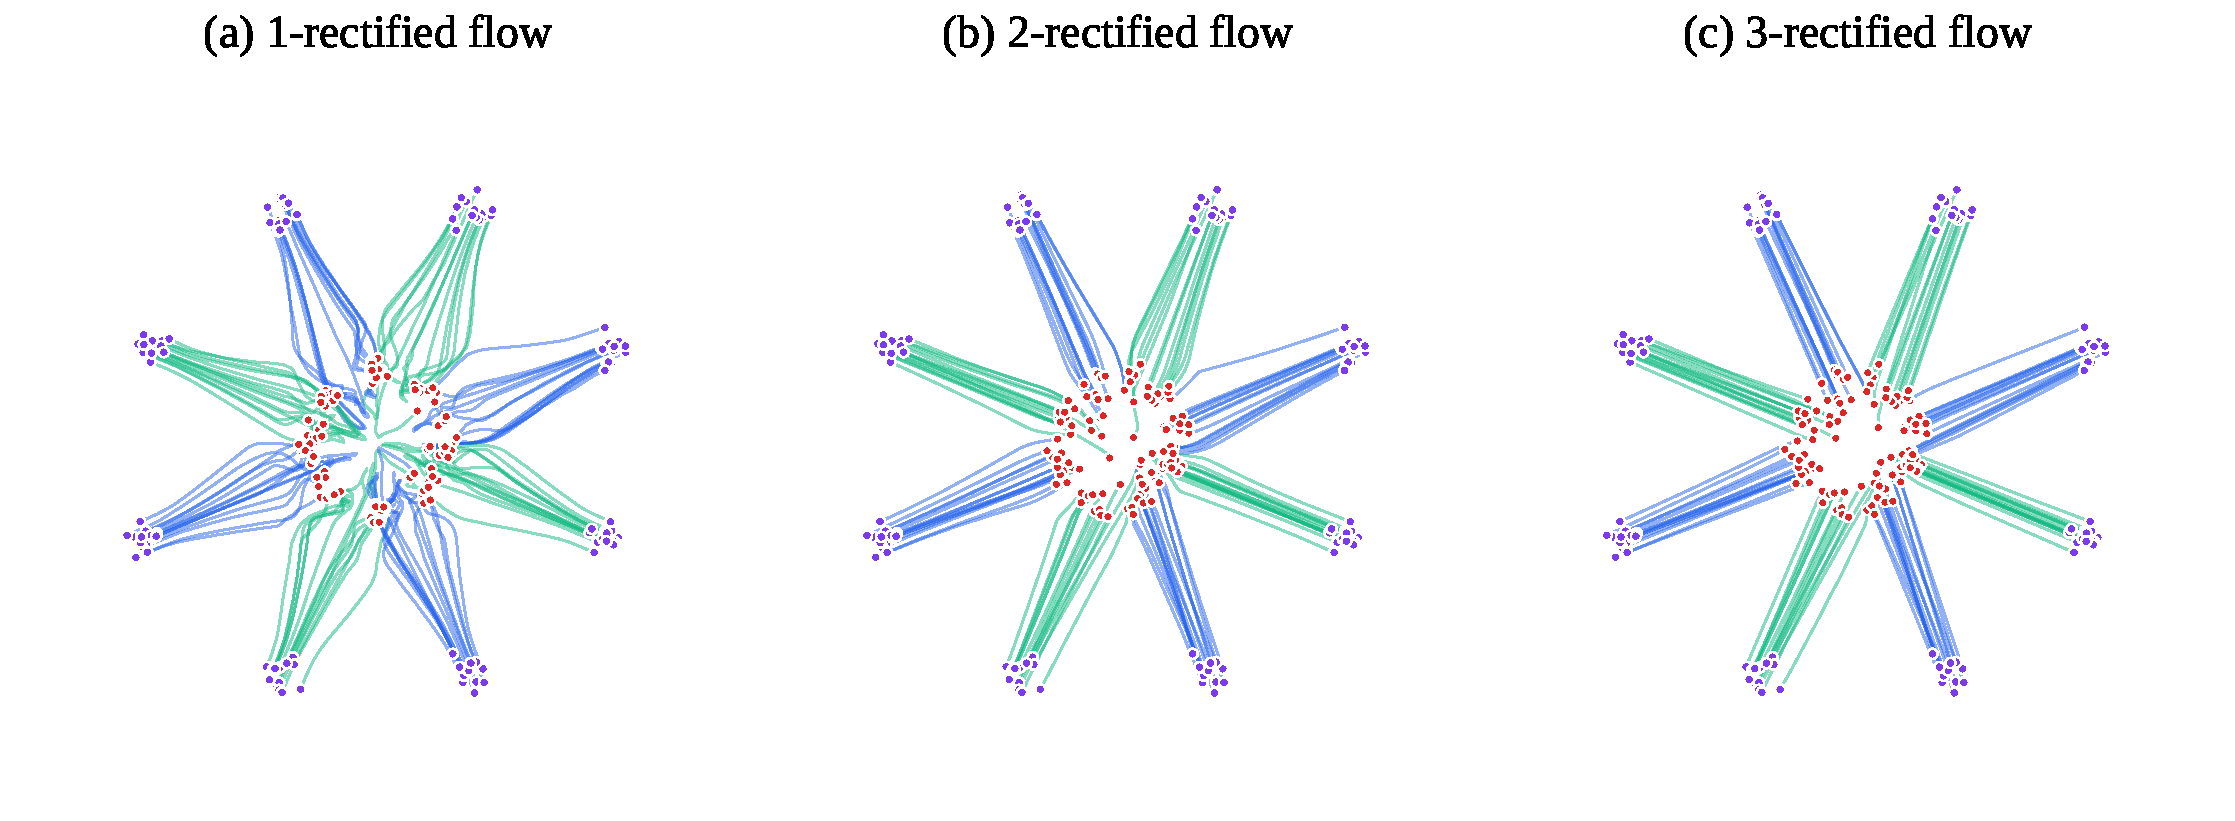
\includegraphics[width=\textwidth]{Images/PartB/rectified_flow_trained.pdf}
    \caption{\textbfs{Illustration of \texttt{Reflow}.} Paths become progressively straighter with \texttt{Rectify} procedure.  \figcredit{Adapted from \citet{liu2022flow}.}}
    \label{fig:ill_Reflow}
\end{figure}


The FM or RF formulation with linear interpolation kernels, together with the \texttt{Reflow} procedure, provides a simpler training objective and a practical method for refining stochastic couplings. For theoretical details, we refer readers to \citep{liu2022flow, liu2022rectified}.



\paragraph{III. Connection to Optimal Transport.}
Lastly, we note that straight-line couplings are not necessarily optimal in the sense of optimal transport (OT). This involves some terminology that will be introduced in \Cref{sec:ot-intro}; we therefore refer readers who are not familiar with OT to that section.

A hallmark of quadratic-cost optimal transport is that particles travel along straight lines: a particle at $\rvx_0$ moves to $\rmT(\rvx_0)$ via $\rvx_t = (1 - t)\rvx_0 + t \rmT(\rvx_0)$, where $\rmT$ is the optimal transport map. However, not every map $\rmS$ generating such straight-line paths, i.e., $\rvx_t = (1 - t)\rvx_0 + t \rmS(\rvx_0)$, is optimal. The map $\rmS$ yields the optimal flow only if it minimizes the Monge cost $\mathbb{E}[\|\rvx_0 - \rmS(\rvx_0)\|^2]$. Thus, while straight-line paths are necessary, they are not sufficient; optimality also depends on the correct endpoint map $\rmT$.

\exm{Straight Couplings Need Not Be Optimal}{
Let $p_{\text{src}} = p_{\text{tgt}} = \mathcal{N}(\bm{0}, \rmI)$. For the cost $c(\rvx, \rvy) = \|\rvx - \rvy\|^p$ with $p > 0$, the $c$-optimal coupling is the identity coupling $\pi^{*}$, where $\pi^{*}$ is the law of $(\rvx, \rvx)$ with $\rvx \sim p_{\text{src}}$.

Now consider the coupling $\pi_{\rmA}$ defined as the law of $(\rvx, \rmA \rvx)$, where $\rvx \sim p_{\text{src}}$ and $\rmA$ is a rotation matrix satisfying $\rmA^\top \rmA = \rmI$, $\det(\rmA) = 1$, $\rmA \neq \rmI$, and $-1$ is not an eigenvalue. Then $\pi_{\rmA}$ is a valid coupling of $p_{\text{src}}$ and $p_{\text{tgt}}$, and corresponds to straight-line paths between $\rvx$ and $\rmA \rvx$, but it is not $c$-optimal for any twice-differentiable strictly convex cost $c$ with invertible Hessian. The suboptimality arises from the rotational transformation. As discussed in \Cref{eq:reflow-loss-gradient}, even removing the rotation may not lead to an optimal coupling.
}

We will continue exploring the connection to OT in \Cref{subsec:ot-linear-reflow}.

\clearpage
\newpage

\newpage
\section{Closing Remarks}\label{sec:ch5_cr}
     
This chapter has illuminated the third and final foundational perspective on diffusion models, one rooted in the principles of deterministic flows. Our exploration began with Normalizing Flows (NFs), which leverage the change-of-variables formula to learn an exact, invertible mapping between a simple prior and the data distribution. We then saw this concept evolve into a continuous-time process with Neural ODEs, where a learned velocity field governs the transformation. However, this approach comes with the significant drawback of requiring costly ODE simulations within the training loop.





The modern framework of Flow Matching (FM) was presented as an elegant and efficient solution to this challenge. By pre-defining a probability path $\{p_{t}\}_t$ and a corresponding velocity field that satisfies the continuity equation, FM establishes a clear target for the ODE flow. Crucially, just as we saw in the variational and score-based views, FM employs a powerful conditioning trick. This transforms the intractable problem of matching the marginal velocity field into a simple and tractable regression against a known conditional velocity, making training entirely simulation-free. This perspective recasts diffusion models themselves as a special case of learning a deterministic flow to transport a Gaussian prior to the data distribution.




With the introduction of the flow-based view, our survey of the three conceptual pillars of diffusion modeling is now complete. Throughout this journey, a remarkable pattern has emerged: each framework, despite its unique origins in VAEs, EBMs, or NFs, has converged on a continuous-time generative process and has relied on a conditioning strategy to enable tractable learning.

In the next chapter, we will finally synthesize these parallel threads into a single, unified framework. We will:
\begin{enumerate}
    \item Formally demonstrate that the variational, score-based, and flow-based perspectives are not merely analogous but are mathematically equivalent at a fundamental level.
    \item Show how the Fokker-Planck equation serves as the universal law governing density evolution across all three views, revealing that they are simply different lenses for describing the same core generative principle.
\end{enumerate}

This unified lens will provide a complete and systematic understanding of the modern diffusion paradigm. 



